\documentclass[conference]{IEEEtran}
\usepackage[utf8]{inputenc}
\usepackage[T1]{fontenc}
\usepackage{amsmath,amssymb}
\usepackage{graphicx}
\usepackage{booktabs}
\usepackage{multirow}
\usepackage{url}
\usepackage{cite}
\usepackage[hidelinks]{hyperref}
% Generated by analysis.security_final.paper_assets from the frozen lock. Do not edit.
\makeatletter
\providecommand{\numdef}[2]{\expandafter\def\csname num@#1\endcsname{#2}}
\providecommand{\val}[1]{\ifcsname num@#1\endcsname\csname num@#1\endcsname\else\textbf{??#1??}\PackageWarning{paper}{missing number #1}\fi}
\numdef{calls.controlled}{570}
\numdef{calls.genpilot}{176}
\numdef{calls.gentest}{4,618}
\numdef{calls.l5pilot}{154}
\numdef{calls.main}{2,919}
\numdef{calls.replay}{516}
\numdef{calls.total}{8,953}
\numdef{ch.A.I.hi}{55.0}
\numdef{ch.A.I.lo}{45.0}
\numdef{ch.A.I.n}{40}
\numdef{ch.A.I.pct}{45.0--55.0}
\numdef{ch.A.I.s}{18}
\numdef{ch.A.I.u}{4}
\numdef{ch.A.P.hi}{64.8}
\numdef{ch.A.P.lo}{35.2}
\numdef{ch.A.P.n}{40}
\numdef{ch.A.P.pct}{50.0}
\numdef{ch.A.P.s}{20}
\numdef{ch.A.P.u}{0}
\numdef{ch.A.attack_correct.hi}{48.5}
\numdef{ch.A.attack_correct.lo}{27.7}
\numdef{ch.A.attack_correct.n}{80}
\numdef{ch.A.attack_correct.pct}{37.5}
\numdef{ch.A.attack_correct.s}{30}
\numdef{ch.A.attack_correct.u}{0}
\numdef{ch.A.attack_correct_without_fake.hi}{49.0}
\numdef{ch.A.attack_correct_without_fake.lo}{27.2}
\numdef{ch.A.attack_correct_without_fake.n}{72}
\numdef{ch.A.attack_correct_without_fake.pct}{37.5}
\numdef{ch.A.attack_correct_without_fake.s}{27}
\numdef{ch.A.attack_correct_without_fake.u}{0}
\numdef{ch.A.attack_two_sources_report_kept.hi}{30.0}
\numdef{ch.A.attack_two_sources_report_kept.lo}{12.0}
\numdef{ch.A.attack_two_sources_report_kept.n}{72}
\numdef{ch.A.attack_two_sources_report_kept.pct}{19.4}
\numdef{ch.A.attack_two_sources_report_kept.s}{14}
\numdef{ch.A.attack_two_sources_report_kept.u}{0}
\numdef{ch.A.clean_correct.hi}{61.9}
\numdef{ch.A.clean_correct.lo}{40.5}
\numdef{ch.A.clean_correct.n}{80}
\numdef{ch.A.clean_correct.pct}{51.2}
\numdef{ch.A.clean_correct.s}{41}
\numdef{ch.A.clean_correct.u}{0}
\numdef{ch.A.clean_refusal.hi}{36.8}
\numdef{ch.A.clean_refusal.lo}{17.9}
\numdef{ch.A.clean_refusal.n}{80}
\numdef{ch.A.clean_refusal.pct}{26.2}
\numdef{ch.A.clean_refusal.s}{21}
\numdef{ch.A.clean_refusal.u}{0}
\numdef{ch.A.src.ai}{5}
\numdef{ch.A.src.human}{66}
\numdef{ch.A.src.scorer}{89}
\numdef{ch.A.total.hi}{52.5}
\numdef{ch.A.total.lo}{47.5}
\numdef{ch.A.total.n}{80}
\numdef{ch.A.total.pct}{47.5--52.5}
\numdef{ch.A.total.s}{38}
\numdef{ch.A.total.u}{4}
\numdef{ch.Apost.I.hi}{23.1}
\numdef{ch.Apost.I.lo}{4.0}
\numdef{ch.Apost.I.n}{40}
\numdef{ch.Apost.I.pct}{10.0}
\numdef{ch.Apost.I.s}{4}
\numdef{ch.Apost.I.u}{0}
\numdef{ch.Apost.P.hi}{16.5}
\numdef{ch.Apost.P.lo}{1.4}
\numdef{ch.Apost.P.n}{40}
\numdef{ch.Apost.P.pct}{5.0}
\numdef{ch.Apost.P.s}{2}
\numdef{ch.Apost.P.u}{0}
\numdef{ch.Apost.attack_correct.hi}{95.7}
\numdef{ch.Apost.attack_correct.lo}{83.0}
\numdef{ch.Apost.attack_correct.n}{80}
\numdef{ch.Apost.attack_correct.pct}{91.2}
\numdef{ch.Apost.attack_correct.s}{73}
\numdef{ch.Apost.attack_correct.u}{0}
\numdef{ch.Apost.attack_correct_without_fake.hi}{93.3}
\numdef{ch.Apost.attack_correct_without_fake.lo}{77.9}
\numdef{ch.Apost.attack_correct_without_fake.n}{72}
\numdef{ch.Apost.attack_correct_without_fake.pct}{87.5}
\numdef{ch.Apost.attack_correct_without_fake.s}{63}
\numdef{ch.Apost.attack_correct_without_fake.u}{0}
\numdef{ch.Apost.attack_two_sources_report_kept.hi}{72.8}
\numdef{ch.Apost.attack_two_sources_report_kept.lo}{51.0}
\numdef{ch.Apost.attack_two_sources_report_kept.n}{72}
\numdef{ch.Apost.attack_two_sources_report_kept.pct}{62.5}
\numdef{ch.Apost.attack_two_sources_report_kept.s}{45}
\numdef{ch.Apost.attack_two_sources_report_kept.u}{0}
\numdef{ch.Apost.clean_correct.hi}{98.7}
\numdef{ch.Apost.clean_correct.lo}{89.5}
\numdef{ch.Apost.clean_correct.n}{80}
\numdef{ch.Apost.clean_correct.pct}{96.2}
\numdef{ch.Apost.clean_correct.s}{77}
\numdef{ch.Apost.clean_correct.u}{0}
\numdef{ch.Apost.clean_refusal.hi}{6.7}
\numdef{ch.Apost.clean_refusal.lo}{0.2}
\numdef{ch.Apost.clean_refusal.n}{80}
\numdef{ch.Apost.clean_refusal.pct}{1.2}
\numdef{ch.Apost.clean_refusal.s}{1}
\numdef{ch.Apost.clean_refusal.u}{0}
\numdef{ch.Apost.src.ai}{17}
\numdef{ch.Apost.src.human}{22}
\numdef{ch.Apost.src.scorer}{121}
\numdef{ch.Apost.total.hi}{15.4}
\numdef{ch.Apost.total.lo}{3.5}
\numdef{ch.Apost.total.n}{80}
\numdef{ch.Apost.total.pct}{7.5}
\numdef{ch.Apost.total.s}{6}
\numdef{ch.Apost.total.u}{0}
\numdef{ch.ApostG.I.hi}{16.5}
\numdef{ch.ApostG.I.lo}{1.4}
\numdef{ch.ApostG.I.n}{40}
\numdef{ch.ApostG.I.pct}{5.0}
\numdef{ch.ApostG.I.s}{2}
\numdef{ch.ApostG.I.u}{0}
\numdef{ch.ApostG.P.hi}{16.5}
\numdef{ch.ApostG.P.lo}{1.4}
\numdef{ch.ApostG.P.n}{40}
\numdef{ch.ApostG.P.pct}{5.0}
\numdef{ch.ApostG.P.s}{2}
\numdef{ch.ApostG.P.u}{0}
\numdef{ch.ApostG.attack_correct.hi}{94.8}
\numdef{ch.ApostG.attack_correct.lo}{81.5}
\numdef{ch.ApostG.attack_correct.n}{80}
\numdef{ch.ApostG.attack_correct.pct}{90.0}
\numdef{ch.ApostG.attack_correct.s}{72}
\numdef{ch.ApostG.attack_correct.u}{0}
\numdef{ch.ApostG.attack_correct_without_fake.hi}{94.3}
\numdef{ch.ApostG.attack_correct_without_fake.lo}{79.6}
\numdef{ch.ApostG.attack_correct_without_fake.n}{72}
\numdef{ch.ApostG.attack_correct_without_fake.pct}{88.9}
\numdef{ch.ApostG.attack_correct_without_fake.s}{64}
\numdef{ch.ApostG.attack_correct_without_fake.u}{0}
\numdef{ch.ApostG.attack_two_sources_report_kept.hi}{71.5}
\numdef{ch.ApostG.attack_two_sources_report_kept.lo}{49.6}
\numdef{ch.ApostG.attack_two_sources_report_kept.n}{72}
\numdef{ch.ApostG.attack_two_sources_report_kept.pct}{61.1}
\numdef{ch.ApostG.attack_two_sources_report_kept.s}{44}
\numdef{ch.ApostG.attack_two_sources_report_kept.u}{0}
\numdef{ch.ApostG.clean_correct.hi}{98.0}
\numdef{ch.ApostG.clean_correct.lo}{87.8}
\numdef{ch.ApostG.clean_correct.n}{80}
\numdef{ch.ApostG.clean_correct.pct}{95.0}
\numdef{ch.ApostG.clean_correct.s}{76}
\numdef{ch.ApostG.clean_correct.u}{0}
\numdef{ch.ApostG.clean_refusal.hi}{6.7}
\numdef{ch.ApostG.clean_refusal.lo}{0.2}
\numdef{ch.ApostG.clean_refusal.n}{80}
\numdef{ch.ApostG.clean_refusal.pct}{1.2}
\numdef{ch.ApostG.clean_refusal.s}{1}
\numdef{ch.ApostG.clean_refusal.u}{0}
\numdef{ch.ApostG.src.ai}{23}
\numdef{ch.ApostG.src.human}{19}
\numdef{ch.ApostG.src.scorer}{118}
\numdef{ch.ApostG.total.hi}{12.2}
\numdef{ch.ApostG.total.lo}{2.0}
\numdef{ch.ApostG.total.n}{80}
\numdef{ch.ApostG.total.pct}{5.0}
\numdef{ch.ApostG.total.s}{4}
\numdef{ch.ApostG.total.u}{0}
\numdef{ch.Apre.I.hi}{32.5}
\numdef{ch.Apre.I.lo}{30.0}
\numdef{ch.Apre.I.n}{40}
\numdef{ch.Apre.I.pct}{30.0--32.5}
\numdef{ch.Apre.I.s}{12}
\numdef{ch.Apre.I.u}{1}
\numdef{ch.Apre.P.hi}{31.9}
\numdef{ch.Apre.P.lo}{8.7}
\numdef{ch.Apre.P.n}{40}
\numdef{ch.Apre.P.pct}{17.5}
\numdef{ch.Apre.P.s}{7}
\numdef{ch.Apre.P.u}{0}
\numdef{ch.Apre.attack_correct.hi}{85.3}
\numdef{ch.Apre.attack_correct.lo}{67.2}
\numdef{ch.Apre.attack_correct.n}{80}
\numdef{ch.Apre.attack_correct.pct}{77.5}
\numdef{ch.Apre.attack_correct.s}{62}
\numdef{ch.Apre.attack_correct.u}{0}
\numdef{ch.Apre.attack_correct_without_fake.hi}{82.4}
\numdef{ch.Apre.attack_correct_without_fake.lo}{62.4}
\numdef{ch.Apre.attack_correct_without_fake.n}{72}
\numdef{ch.Apre.attack_correct_without_fake.pct}{73.6}
\numdef{ch.Apre.attack_correct_without_fake.s}{53}
\numdef{ch.Apre.attack_correct_without_fake.u}{0}
\numdef{ch.Apre.attack_two_sources_report_kept.hi}{51.8}
\numdef{ch.Apre.attack_two_sources_report_kept.lo}{29.7}
\numdef{ch.Apre.attack_two_sources_report_kept.n}{72}
\numdef{ch.Apre.attack_two_sources_report_kept.pct}{40.3}
\numdef{ch.Apre.attack_two_sources_report_kept.s}{29}
\numdef{ch.Apre.attack_two_sources_report_kept.u}{0}
\numdef{ch.Apre.clean_correct.hi}{97.3}
\numdef{ch.Apre.clean_correct.lo}{86.2}
\numdef{ch.Apre.clean_correct.n}{80}
\numdef{ch.Apre.clean_correct.pct}{93.8}
\numdef{ch.Apre.clean_correct.s}{75}
\numdef{ch.Apre.clean_correct.u}{0}
\numdef{ch.Apre.clean_refusal.hi}{6.7}
\numdef{ch.Apre.clean_refusal.lo}{0.2}
\numdef{ch.Apre.clean_refusal.n}{80}
\numdef{ch.Apre.clean_refusal.pct}{1.2}
\numdef{ch.Apre.clean_refusal.s}{1}
\numdef{ch.Apre.clean_refusal.u}{0}
\numdef{ch.Apre.src.ai}{15}
\numdef{ch.Apre.src.human}{18}
\numdef{ch.Apre.src.scorer}{127}
\numdef{ch.Apre.total.hi}{25.0}
\numdef{ch.Apre.total.lo}{23.8}
\numdef{ch.Apre.total.n}{80}
\numdef{ch.Apre.total.pct}{23.8--25.0}
\numdef{ch.Apre.total.s}{19}
\numdef{ch.Apre.total.u}{1}
\numdef{ch.D.I.cp}{8.8}
\numdef{ch.D.I.hi}{8.8}
\numdef{ch.D.I.lo}{0.0}
\numdef{ch.D.I.n}{40}
\numdef{ch.D.I.pct}{0.0}
\numdef{ch.D.I.s}{0}
\numdef{ch.D.I.u}{0}
\numdef{ch.D.P.cp}{8.8}
\numdef{ch.D.P.hi}{8.8}
\numdef{ch.D.P.lo}{0.0}
\numdef{ch.D.P.n}{40}
\numdef{ch.D.P.pct}{0.0}
\numdef{ch.D.P.s}{0}
\numdef{ch.D.P.u}{0}
\numdef{ch.D.attack_correct.hi}{96.5}
\numdef{ch.D.attack_correct.lo}{84.6}
\numdef{ch.D.attack_correct.n}{80}
\numdef{ch.D.attack_correct.pct}{92.5}
\numdef{ch.D.attack_correct.s}{74}
\numdef{ch.D.attack_correct.u}{0}
\numdef{ch.D.attack_correct_without_fake.hi}{96.1}
\numdef{ch.D.attack_correct_without_fake.lo}{83.0}
\numdef{ch.D.attack_correct_without_fake.n}{72}
\numdef{ch.D.attack_correct_without_fake.pct}{91.7}
\numdef{ch.D.attack_correct_without_fake.s}{66}
\numdef{ch.D.attack_correct_without_fake.u}{0}
\numdef{ch.D.attack_two_sources_report_kept.hi}{53.2}
\numdef{ch.D.attack_two_sources_report_kept.lo}{31.0}
\numdef{ch.D.attack_two_sources_report_kept.n}{72}
\numdef{ch.D.attack_two_sources_report_kept.pct}{41.7}
\numdef{ch.D.attack_two_sources_report_kept.s}{30}
\numdef{ch.D.attack_two_sources_report_kept.u}{0}
\numdef{ch.D.clean_correct.hi}{99.3}
\numdef{ch.D.clean_correct.lo}{91.3}
\numdef{ch.D.clean_correct.n}{80}
\numdef{ch.D.clean_correct.pct}{97.5}
\numdef{ch.D.clean_correct.s}{78}
\numdef{ch.D.clean_correct.u}{0}
\numdef{ch.D.clean_refusal.hi}{4.6}
\numdef{ch.D.clean_refusal.lo}{0.0}
\numdef{ch.D.clean_refusal.n}{80}
\numdef{ch.D.clean_refusal.pct}{0.0}
\numdef{ch.D.clean_refusal.s}{0}
\numdef{ch.D.clean_refusal.u}{0}
\numdef{ch.D.src.ai}{11}
\numdef{ch.D.src.human}{17}
\numdef{ch.D.src.scorer}{132}
\numdef{ch.D.total.cp}{4.5}
\numdef{ch.D.total.hi}{4.6}
\numdef{ch.D.total.lo}{0.0}
\numdef{ch.D.total.n}{80}
\numdef{ch.D.total.pct}{0.0}
\numdef{ch.D.total.s}{0}
\numdef{ch.D.total.u}{0}
\numdef{ch.sens.A.I.hi}{55.0}
\numdef{ch.sens.A.I.lo}{45.0}
\numdef{ch.sens.A.I.n}{40}
\numdef{ch.sens.A.I.pct}{45.0--55.0}
\numdef{ch.sens.A.I.s}{18}
\numdef{ch.sens.A.I.u}{4}
\numdef{ch.sens.A.P.hi}{64.8}
\numdef{ch.sens.A.P.lo}{35.2}
\numdef{ch.sens.A.P.n}{40}
\numdef{ch.sens.A.P.pct}{50.0}
\numdef{ch.sens.A.P.s}{20}
\numdef{ch.sens.A.P.u}{0}
\numdef{ch.sens.A.total.hi}{52.5}
\numdef{ch.sens.A.total.lo}{47.5}
\numdef{ch.sens.A.total.n}{80}
\numdef{ch.sens.A.total.pct}{47.5--52.5}
\numdef{ch.sens.A.total.s}{38}
\numdef{ch.sens.A.total.u}{4}
\numdef{ch.sens.Apost.I.hi}{23.1}
\numdef{ch.sens.Apost.I.lo}{4.0}
\numdef{ch.sens.Apost.I.n}{40}
\numdef{ch.sens.Apost.I.pct}{10.0}
\numdef{ch.sens.Apost.I.s}{4}
\numdef{ch.sens.Apost.I.u}{0}
\numdef{ch.sens.Apost.P.hi}{16.5}
\numdef{ch.sens.Apost.P.lo}{1.4}
\numdef{ch.sens.Apost.P.n}{40}
\numdef{ch.sens.Apost.P.pct}{5.0}
\numdef{ch.sens.Apost.P.s}{2}
\numdef{ch.sens.Apost.P.u}{0}
\numdef{ch.sens.Apost.total.hi}{15.4}
\numdef{ch.sens.Apost.total.lo}{3.5}
\numdef{ch.sens.Apost.total.n}{80}
\numdef{ch.sens.Apost.total.pct}{7.5}
\numdef{ch.sens.Apost.total.s}{6}
\numdef{ch.sens.Apost.total.u}{0}
\numdef{ch.sens.ApostG.I.hi}{16.5}
\numdef{ch.sens.ApostG.I.lo}{1.4}
\numdef{ch.sens.ApostG.I.n}{40}
\numdef{ch.sens.ApostG.I.pct}{5.0}
\numdef{ch.sens.ApostG.I.s}{2}
\numdef{ch.sens.ApostG.I.u}{0}
\numdef{ch.sens.ApostG.P.hi}{16.5}
\numdef{ch.sens.ApostG.P.lo}{1.4}
\numdef{ch.sens.ApostG.P.n}{40}
\numdef{ch.sens.ApostG.P.pct}{5.0}
\numdef{ch.sens.ApostG.P.s}{2}
\numdef{ch.sens.ApostG.P.u}{0}
\numdef{ch.sens.ApostG.total.hi}{12.2}
\numdef{ch.sens.ApostG.total.lo}{2.0}
\numdef{ch.sens.ApostG.total.n}{80}
\numdef{ch.sens.ApostG.total.pct}{5.0}
\numdef{ch.sens.ApostG.total.s}{4}
\numdef{ch.sens.ApostG.total.u}{0}
\numdef{ch.sens.Apre.I.hi}{32.5}
\numdef{ch.sens.Apre.I.lo}{30.0}
\numdef{ch.sens.Apre.I.n}{40}
\numdef{ch.sens.Apre.I.pct}{30.0--32.5}
\numdef{ch.sens.Apre.I.s}{12}
\numdef{ch.sens.Apre.I.u}{1}
\numdef{ch.sens.Apre.P.hi}{31.9}
\numdef{ch.sens.Apre.P.lo}{8.7}
\numdef{ch.sens.Apre.P.n}{40}
\numdef{ch.sens.Apre.P.pct}{17.5}
\numdef{ch.sens.Apre.P.s}{7}
\numdef{ch.sens.Apre.P.u}{0}
\numdef{ch.sens.Apre.total.hi}{25.0}
\numdef{ch.sens.Apre.total.lo}{23.8}
\numdef{ch.sens.Apre.total.n}{80}
\numdef{ch.sens.Apre.total.pct}{23.8--25.0}
\numdef{ch.sens.Apre.total.s}{19}
\numdef{ch.sens.Apre.total.u}{1}
\numdef{ch.sens.D.I.cp}{8.8}
\numdef{ch.sens.D.I.hi}{8.8}
\numdef{ch.sens.D.I.lo}{0.0}
\numdef{ch.sens.D.I.n}{40}
\numdef{ch.sens.D.I.pct}{0.0}
\numdef{ch.sens.D.I.s}{0}
\numdef{ch.sens.D.I.u}{0}
\numdef{ch.sens.D.P.cp}{8.8}
\numdef{ch.sens.D.P.hi}{8.8}
\numdef{ch.sens.D.P.lo}{0.0}
\numdef{ch.sens.D.P.n}{40}
\numdef{ch.sens.D.P.pct}{0.0}
\numdef{ch.sens.D.P.s}{0}
\numdef{ch.sens.D.P.u}{0}
\numdef{ch.sens.D.total.cp}{4.5}
\numdef{ch.sens.D.total.hi}{4.6}
\numdef{ch.sens.D.total.lo}{0.0}
\numdef{ch.sens.D.total.n}{80}
\numdef{ch.sens.D.total.pct}{0.0}
\numdef{ch.sens.D.total.s}{0}
\numdef{ch.sens.D.total.u}{0}
\numdef{ch.test.all.AApre.a}{28}
\numdef{ch.test.all.AApre.b}{7}
\numdef{ch.test.all.AApre.n}{75}
\numdef{ch.test.all.AApre.p}{\ensuremath{5.1{\times}10^{-4}}}
\numdef{ch.test.all.AApre.ph}{0.00203}
\numdef{ch.test.all.AApre.u}{5}
\numdef{ch.test.all.ApostApostG.a}{3}
\numdef{ch.test.all.ApostApostG.b}{1}
\numdef{ch.test.all.ApostApostG.n}{80}
\numdef{ch.test.all.ApostApostG.p}{0.625}
\numdef{ch.test.all.ApostApostG.ph}{0.625}
\numdef{ch.test.all.ApostApostG.u}{0}
\numdef{ch.test.all.ApostD.a}{6}
\numdef{ch.test.all.ApostD.b}{0}
\numdef{ch.test.all.ApostD.n}{80}
\numdef{ch.test.all.ApostD.p}{0.0312}
\numdef{ch.test.all.ApostD.ph}{0.0625}
\numdef{ch.test.all.ApostD.u}{0}
\numdef{ch.test.all.ApreApost.a}{15}
\numdef{ch.test.all.ApreApost.b}{2}
\numdef{ch.test.all.ApreApost.n}{79}
\numdef{ch.test.all.ApreApost.p}{0.00235}
\numdef{ch.test.all.ApreApost.ph}{0.00705}
\numdef{ch.test.all.ApreApost.u}{1}
\numdef{g.aiai.items}{84}
\numdef{g.aiai.match}{62}
\numdef{g.dsucc.main}{2}
\numdef{g.gemma4-31b.A.I.hi}{55.0}
\numdef{g.gemma4-31b.A.I.lo}{45.0}
\numdef{g.gemma4-31b.A.I.n}{40}
\numdef{g.gemma4-31b.A.I.pct}{45.0--55.0}
\numdef{g.gemma4-31b.A.I.s}{18}
\numdef{g.gemma4-31b.A.I.u}{4}
\numdef{g.gemma4-31b.A.P.hi}{62.5}
\numdef{g.gemma4-31b.A.P.lo}{32.9}
\numdef{g.gemma4-31b.A.P.n}{40}
\numdef{g.gemma4-31b.A.P.pct}{47.5}
\numdef{g.gemma4-31b.A.P.s}{19}
\numdef{g.gemma4-31b.A.P.u}{0}
\numdef{g.gemma4-31b.A.attack_correct.hi}{51.0}
\numdef{g.gemma4-31b.A.attack_correct.lo}{30.0}
\numdef{g.gemma4-31b.A.attack_correct.n}{80}
\numdef{g.gemma4-31b.A.attack_correct.pct}{40.0}
\numdef{g.gemma4-31b.A.attack_correct.s}{32}
\numdef{g.gemma4-31b.A.attack_correct.u}{0}
\numdef{g.gemma4-31b.A.attack_correct_without_fake.hi}{54.6}
\numdef{g.gemma4-31b.A.attack_correct_without_fake.lo}{32.3}
\numdef{g.gemma4-31b.A.attack_correct_without_fake.n}{72}
\numdef{g.gemma4-31b.A.attack_correct_without_fake.pct}{43.1}
\numdef{g.gemma4-31b.A.attack_correct_without_fake.s}{31}
\numdef{g.gemma4-31b.A.attack_correct_without_fake.u}{0}
\numdef{g.gemma4-31b.A.attack_two_sources_report_kept.hi}{37.6}
\numdef{g.gemma4-31b.A.attack_two_sources_report_kept.lo}{17.6}
\numdef{g.gemma4-31b.A.attack_two_sources_report_kept.n}{72}
\numdef{g.gemma4-31b.A.attack_two_sources_report_kept.pct}{26.4}
\numdef{g.gemma4-31b.A.attack_two_sources_report_kept.s}{19}
\numdef{g.gemma4-31b.A.attack_two_sources_report_kept.u}{0}
\numdef{g.gemma4-31b.A.clean_correct.hi}{63.1}
\numdef{g.gemma4-31b.A.clean_correct.lo}{41.7}
\numdef{g.gemma4-31b.A.clean_correct.n}{80}
\numdef{g.gemma4-31b.A.clean_correct.pct}{52.5}
\numdef{g.gemma4-31b.A.clean_correct.s}{42}
\numdef{g.gemma4-31b.A.clean_correct.u}{0}
\numdef{g.gemma4-31b.A.clean_refusal.hi}{52.2}
\numdef{g.gemma4-31b.A.clean_refusal.lo}{31.1}
\numdef{g.gemma4-31b.A.clean_refusal.n}{80}
\numdef{g.gemma4-31b.A.clean_refusal.pct}{41.2}
\numdef{g.gemma4-31b.A.clean_refusal.s}{33}
\numdef{g.gemma4-31b.A.clean_refusal.u}{0}
\numdef{g.gemma4-31b.A.total.hi}{51.2}
\numdef{g.gemma4-31b.A.total.lo}{46.2}
\numdef{g.gemma4-31b.A.total.n}{80}
\numdef{g.gemma4-31b.A.total.pct}{46.2--51.2}
\numdef{g.gemma4-31b.A.total.s}{37}
\numdef{g.gemma4-31b.A.total.u}{4}
\numdef{g.gemma4-31b.D.I.cp}{8.8}
\numdef{g.gemma4-31b.D.I.hi}{8.8}
\numdef{g.gemma4-31b.D.I.lo}{0.0}
\numdef{g.gemma4-31b.D.I.n}{40}
\numdef{g.gemma4-31b.D.I.pct}{0.0}
\numdef{g.gemma4-31b.D.I.s}{0}
\numdef{g.gemma4-31b.D.I.u}{0}
\numdef{g.gemma4-31b.D.P.cp}{8.8}
\numdef{g.gemma4-31b.D.P.hi}{8.8}
\numdef{g.gemma4-31b.D.P.lo}{0.0}
\numdef{g.gemma4-31b.D.P.n}{40}
\numdef{g.gemma4-31b.D.P.pct}{0.0}
\numdef{g.gemma4-31b.D.P.s}{0}
\numdef{g.gemma4-31b.D.P.u}{0}
\numdef{g.gemma4-31b.D.attack_correct.hi}{94.8}
\numdef{g.gemma4-31b.D.attack_correct.lo}{81.5}
\numdef{g.gemma4-31b.D.attack_correct.n}{80}
\numdef{g.gemma4-31b.D.attack_correct.pct}{90.0}
\numdef{g.gemma4-31b.D.attack_correct.s}{72}
\numdef{g.gemma4-31b.D.attack_correct.u}{0}
\numdef{g.gemma4-31b.D.attack_correct_without_fake.hi}{94.3}
\numdef{g.gemma4-31b.D.attack_correct_without_fake.lo}{79.6}
\numdef{g.gemma4-31b.D.attack_correct_without_fake.n}{72}
\numdef{g.gemma4-31b.D.attack_correct_without_fake.pct}{88.9}
\numdef{g.gemma4-31b.D.attack_correct_without_fake.s}{64}
\numdef{g.gemma4-31b.D.attack_correct_without_fake.u}{0}
\numdef{g.gemma4-31b.D.attack_two_sources_report_kept.hi}{37.6}
\numdef{g.gemma4-31b.D.attack_two_sources_report_kept.lo}{17.6}
\numdef{g.gemma4-31b.D.attack_two_sources_report_kept.n}{72}
\numdef{g.gemma4-31b.D.attack_two_sources_report_kept.pct}{26.4}
\numdef{g.gemma4-31b.D.attack_two_sources_report_kept.s}{19}
\numdef{g.gemma4-31b.D.attack_two_sources_report_kept.u}{0}
\numdef{g.gemma4-31b.D.clean_correct.hi}{95.7}
\numdef{g.gemma4-31b.D.clean_correct.lo}{83.0}
\numdef{g.gemma4-31b.D.clean_correct.n}{80}
\numdef{g.gemma4-31b.D.clean_correct.pct}{91.2}
\numdef{g.gemma4-31b.D.clean_correct.s}{73}
\numdef{g.gemma4-31b.D.clean_correct.u}{0}
\numdef{g.gemma4-31b.D.clean_refusal.hi}{12.2}
\numdef{g.gemma4-31b.D.clean_refusal.lo}{2.0}
\numdef{g.gemma4-31b.D.clean_refusal.n}{80}
\numdef{g.gemma4-31b.D.clean_refusal.pct}{5.0}
\numdef{g.gemma4-31b.D.clean_refusal.s}{4}
\numdef{g.gemma4-31b.D.clean_refusal.u}{0}
\numdef{g.gemma4-31b.D.total.cp}{4.5}
\numdef{g.gemma4-31b.D.total.hi}{4.6}
\numdef{g.gemma4-31b.D.total.lo}{0.0}
\numdef{g.gemma4-31b.D.total.n}{80}
\numdef{g.gemma4-31b.D.total.pct}{0.0}
\numdef{g.gemma4-31b.D.total.s}{0}
\numdef{g.gemma4-31b.D.total.u}{0}
\numdef{g.gemma4-31b.calls}{1,633}
\numdef{g.gemma4-31b.sens.A.I.hi}{55.0}
\numdef{g.gemma4-31b.sens.A.I.lo}{45.0}
\numdef{g.gemma4-31b.sens.A.I.n}{40}
\numdef{g.gemma4-31b.sens.A.I.pct}{45.0--55.0}
\numdef{g.gemma4-31b.sens.A.I.s}{18}
\numdef{g.gemma4-31b.sens.A.I.u}{4}
\numdef{g.gemma4-31b.sens.A.P.hi}{64.8}
\numdef{g.gemma4-31b.sens.A.P.lo}{35.2}
\numdef{g.gemma4-31b.sens.A.P.n}{40}
\numdef{g.gemma4-31b.sens.A.P.pct}{50.0}
\numdef{g.gemma4-31b.sens.A.P.s}{20}
\numdef{g.gemma4-31b.sens.A.P.u}{0}
\numdef{g.gemma4-31b.sens.A.total.hi}{52.5}
\numdef{g.gemma4-31b.sens.A.total.lo}{47.5}
\numdef{g.gemma4-31b.sens.A.total.n}{80}
\numdef{g.gemma4-31b.sens.A.total.pct}{47.5--52.5}
\numdef{g.gemma4-31b.sens.A.total.s}{38}
\numdef{g.gemma4-31b.sens.A.total.u}{4}
\numdef{g.gemma4-31b.sens.D.I.cp}{8.8}
\numdef{g.gemma4-31b.sens.D.I.hi}{8.8}
\numdef{g.gemma4-31b.sens.D.I.lo}{0.0}
\numdef{g.gemma4-31b.sens.D.I.n}{40}
\numdef{g.gemma4-31b.sens.D.I.pct}{0.0}
\numdef{g.gemma4-31b.sens.D.I.s}{0}
\numdef{g.gemma4-31b.sens.D.I.u}{0}
\numdef{g.gemma4-31b.sens.D.P.cp}{8.8}
\numdef{g.gemma4-31b.sens.D.P.hi}{8.8}
\numdef{g.gemma4-31b.sens.D.P.lo}{0.0}
\numdef{g.gemma4-31b.sens.D.P.n}{40}
\numdef{g.gemma4-31b.sens.D.P.pct}{0.0}
\numdef{g.gemma4-31b.sens.D.P.s}{0}
\numdef{g.gemma4-31b.sens.D.P.u}{0}
\numdef{g.gemma4-31b.sens.D.total.cp}{4.5}
\numdef{g.gemma4-31b.sens.D.total.hi}{4.6}
\numdef{g.gemma4-31b.sens.D.total.lo}{0.0}
\numdef{g.gemma4-31b.sens.D.total.n}{80}
\numdef{g.gemma4-31b.sens.D.total.pct}{0.0}
\numdef{g.gemma4-31b.sens.D.total.s}{0}
\numdef{g.gemma4-31b.sens.D.total.u}{0}
\numdef{g.gemma4-31b.stab.Aruns}{7, 7, 8}
\numdef{g.gemma4-31b.stab.Druns}{0, 0, 0}
\numdef{g.gemma4-31b.stab.changed}{1}
\numdef{g.gemma4-31b.stab.changedD}{0}
\numdef{g.gemma4-31b.stab.pairs}{32}
\numdef{g.gemma4-31b.stab.same}{31}
\numdef{g.gemma4-31b.test.I.a}{18}
\numdef{g.gemma4-31b.test.I.b}{0}
\numdef{g.gemma4-31b.test.I.n}{36}
\numdef{g.gemma4-31b.test.I.p}{\ensuremath{7.6{\times}10^{-6}}}
\numdef{g.gemma4-31b.test.I.ph}{\ensuremath{2.3{\times}10^{-5}}}
\numdef{g.gemma4-31b.test.I.u}{4}
\numdef{g.gemma4-31b.test.P.a}{19}
\numdef{g.gemma4-31b.test.P.b}{0}
\numdef{g.gemma4-31b.test.P.n}{40}
\numdef{g.gemma4-31b.test.P.p}{\ensuremath{3.8{\times}10^{-6}}}
\numdef{g.gemma4-31b.test.P.ph}{\ensuremath{1.5{\times}10^{-5}}}
\numdef{g.gemma4-31b.test.P.u}{0}
\numdef{g.gemma4-31b.valid}{448/448}
\numdef{g.gpt-oss-120b.A.I.hi}{55.0}
\numdef{g.gpt-oss-120b.A.I.lo}{45.0}
\numdef{g.gpt-oss-120b.A.I.n}{40}
\numdef{g.gpt-oss-120b.A.I.pct}{45.0--55.0}
\numdef{g.gpt-oss-120b.A.I.s}{18}
\numdef{g.gpt-oss-120b.A.I.u}{4}
\numdef{g.gpt-oss-120b.A.P.hi}{69.3}
\numdef{g.gpt-oss-120b.A.P.lo}{39.8}
\numdef{g.gpt-oss-120b.A.P.n}{40}
\numdef{g.gpt-oss-120b.A.P.pct}{55.0}
\numdef{g.gpt-oss-120b.A.P.s}{22}
\numdef{g.gpt-oss-120b.A.P.u}{0}
\numdef{g.gpt-oss-120b.A.attack_correct.hi}{52.2}
\numdef{g.gpt-oss-120b.A.attack_correct.lo}{31.1}
\numdef{g.gpt-oss-120b.A.attack_correct.n}{80}
\numdef{g.gpt-oss-120b.A.attack_correct.pct}{41.2}
\numdef{g.gpt-oss-120b.A.attack_correct.s}{33}
\numdef{g.gpt-oss-120b.A.attack_correct.u}{0}
\numdef{g.gpt-oss-120b.A.attack_correct_without_fake.hi}{53.2}
\numdef{g.gpt-oss-120b.A.attack_correct_without_fake.lo}{31.0}
\numdef{g.gpt-oss-120b.A.attack_correct_without_fake.n}{72}
\numdef{g.gpt-oss-120b.A.attack_correct_without_fake.pct}{41.7}
\numdef{g.gpt-oss-120b.A.attack_correct_without_fake.s}{30}
\numdef{g.gpt-oss-120b.A.attack_correct_without_fake.u}{0}
\numdef{g.gpt-oss-120b.A.attack_two_sources_report_kept.hi}{28.5}
\numdef{g.gpt-oss-120b.A.attack_two_sources_report_kept.lo}{10.9}
\numdef{g.gpt-oss-120b.A.attack_two_sources_report_kept.n}{72}
\numdef{g.gpt-oss-120b.A.attack_two_sources_report_kept.pct}{18.1}
\numdef{g.gpt-oss-120b.A.attack_two_sources_report_kept.s}{13}
\numdef{g.gpt-oss-120b.A.attack_two_sources_report_kept.u}{0}
\numdef{g.gpt-oss-120b.A.clean_correct.hi}{60.7}
\numdef{g.gpt-oss-120b.A.clean_correct.lo}{39.3}
\numdef{g.gpt-oss-120b.A.clean_correct.n}{80}
\numdef{g.gpt-oss-120b.A.clean_correct.pct}{50.0}
\numdef{g.gpt-oss-120b.A.clean_correct.s}{40}
\numdef{g.gpt-oss-120b.A.clean_correct.u}{0}
\numdef{g.gpt-oss-120b.A.clean_refusal.hi}{39.5}
\numdef{g.gpt-oss-120b.A.clean_refusal.lo}{20.0}
\numdef{g.gpt-oss-120b.A.clean_refusal.n}{80}
\numdef{g.gpt-oss-120b.A.clean_refusal.pct}{28.7}
\numdef{g.gpt-oss-120b.A.clean_refusal.s}{23}
\numdef{g.gpt-oss-120b.A.clean_refusal.u}{0}
\numdef{g.gpt-oss-120b.A.total.hi}{55.0}
\numdef{g.gpt-oss-120b.A.total.lo}{50.0}
\numdef{g.gpt-oss-120b.A.total.n}{80}
\numdef{g.gpt-oss-120b.A.total.pct}{50.0--55.0}
\numdef{g.gpt-oss-120b.A.total.s}{40}
\numdef{g.gpt-oss-120b.A.total.u}{4}
\numdef{g.gpt-oss-120b.D.I.cp}{8.8}
\numdef{g.gpt-oss-120b.D.I.hi}{8.8}
\numdef{g.gpt-oss-120b.D.I.lo}{0.0}
\numdef{g.gpt-oss-120b.D.I.n}{40}
\numdef{g.gpt-oss-120b.D.I.pct}{0.0}
\numdef{g.gpt-oss-120b.D.I.s}{0}
\numdef{g.gpt-oss-120b.D.I.u}{0}
\numdef{g.gpt-oss-120b.D.P.hi}{12.9}
\numdef{g.gpt-oss-120b.D.P.lo}{0.4}
\numdef{g.gpt-oss-120b.D.P.n}{40}
\numdef{g.gpt-oss-120b.D.P.pct}{2.5}
\numdef{g.gpt-oss-120b.D.P.s}{1}
\numdef{g.gpt-oss-120b.D.P.u}{0}
\numdef{g.gpt-oss-120b.D.attack_correct.hi}{98.0}
\numdef{g.gpt-oss-120b.D.attack_correct.lo}{87.8}
\numdef{g.gpt-oss-120b.D.attack_correct.n}{80}
\numdef{g.gpt-oss-120b.D.attack_correct.pct}{95.0}
\numdef{g.gpt-oss-120b.D.attack_correct.s}{76}
\numdef{g.gpt-oss-120b.D.attack_correct.u}{0}
\numdef{g.gpt-oss-120b.D.attack_correct_without_fake.hi}{97.8}
\numdef{g.gpt-oss-120b.D.attack_correct_without_fake.lo}{86.6}
\numdef{g.gpt-oss-120b.D.attack_correct_without_fake.n}{72}
\numdef{g.gpt-oss-120b.D.attack_correct_without_fake.pct}{94.4}
\numdef{g.gpt-oss-120b.D.attack_correct_without_fake.s}{68}
\numdef{g.gpt-oss-120b.D.attack_correct_without_fake.u}{0}
\numdef{g.gpt-oss-120b.D.attack_two_sources_report_kept.hi}{58.6}
\numdef{g.gpt-oss-120b.D.attack_two_sources_report_kept.lo}{36.1}
\numdef{g.gpt-oss-120b.D.attack_two_sources_report_kept.n}{72}
\numdef{g.gpt-oss-120b.D.attack_two_sources_report_kept.pct}{47.2}
\numdef{g.gpt-oss-120b.D.attack_two_sources_report_kept.s}{34}
\numdef{g.gpt-oss-120b.D.attack_two_sources_report_kept.u}{0}
\numdef{g.gpt-oss-120b.D.clean_correct.hi}{98.0}
\numdef{g.gpt-oss-120b.D.clean_correct.lo}{87.8}
\numdef{g.gpt-oss-120b.D.clean_correct.n}{80}
\numdef{g.gpt-oss-120b.D.clean_correct.pct}{95.0}
\numdef{g.gpt-oss-120b.D.clean_correct.s}{76}
\numdef{g.gpt-oss-120b.D.clean_correct.u}{0}
\numdef{g.gpt-oss-120b.D.clean_refusal.hi}{10.5}
\numdef{g.gpt-oss-120b.D.clean_refusal.lo}{1.3}
\numdef{g.gpt-oss-120b.D.clean_refusal.n}{80}
\numdef{g.gpt-oss-120b.D.clean_refusal.pct}{3.8}
\numdef{g.gpt-oss-120b.D.clean_refusal.s}{3}
\numdef{g.gpt-oss-120b.D.clean_refusal.u}{0}
\numdef{g.gpt-oss-120b.D.total.hi}{6.7}
\numdef{g.gpt-oss-120b.D.total.lo}{0.2}
\numdef{g.gpt-oss-120b.D.total.n}{80}
\numdef{g.gpt-oss-120b.D.total.pct}{1.2}
\numdef{g.gpt-oss-120b.D.total.s}{1}
\numdef{g.gpt-oss-120b.D.total.u}{0}
\numdef{g.gpt-oss-120b.calls}{1,495}
\numdef{g.gpt-oss-120b.sens.A.I.hi}{55.0}
\numdef{g.gpt-oss-120b.sens.A.I.lo}{45.0}
\numdef{g.gpt-oss-120b.sens.A.I.n}{40}
\numdef{g.gpt-oss-120b.sens.A.I.pct}{45.0--55.0}
\numdef{g.gpt-oss-120b.sens.A.I.s}{18}
\numdef{g.gpt-oss-120b.sens.A.I.u}{4}
\numdef{g.gpt-oss-120b.sens.A.P.hi}{67.1}
\numdef{g.gpt-oss-120b.sens.A.P.lo}{37.5}
\numdef{g.gpt-oss-120b.sens.A.P.n}{40}
\numdef{g.gpt-oss-120b.sens.A.P.pct}{52.5}
\numdef{g.gpt-oss-120b.sens.A.P.s}{21}
\numdef{g.gpt-oss-120b.sens.A.P.u}{0}
\numdef{g.gpt-oss-120b.sens.A.total.hi}{53.8}
\numdef{g.gpt-oss-120b.sens.A.total.lo}{48.8}
\numdef{g.gpt-oss-120b.sens.A.total.n}{80}
\numdef{g.gpt-oss-120b.sens.A.total.pct}{48.8--53.8}
\numdef{g.gpt-oss-120b.sens.A.total.s}{39}
\numdef{g.gpt-oss-120b.sens.A.total.u}{4}
\numdef{g.gpt-oss-120b.sens.D.I.cp}{8.8}
\numdef{g.gpt-oss-120b.sens.D.I.hi}{8.8}
\numdef{g.gpt-oss-120b.sens.D.I.lo}{0.0}
\numdef{g.gpt-oss-120b.sens.D.I.n}{40}
\numdef{g.gpt-oss-120b.sens.D.I.pct}{0.0}
\numdef{g.gpt-oss-120b.sens.D.I.s}{0}
\numdef{g.gpt-oss-120b.sens.D.I.u}{0}
\numdef{g.gpt-oss-120b.sens.D.P.cp}{8.8}
\numdef{g.gpt-oss-120b.sens.D.P.hi}{8.8}
\numdef{g.gpt-oss-120b.sens.D.P.lo}{0.0}
\numdef{g.gpt-oss-120b.sens.D.P.n}{40}
\numdef{g.gpt-oss-120b.sens.D.P.pct}{0.0}
\numdef{g.gpt-oss-120b.sens.D.P.s}{0}
\numdef{g.gpt-oss-120b.sens.D.P.u}{0}
\numdef{g.gpt-oss-120b.sens.D.total.cp}{4.5}
\numdef{g.gpt-oss-120b.sens.D.total.hi}{4.6}
\numdef{g.gpt-oss-120b.sens.D.total.lo}{0.0}
\numdef{g.gpt-oss-120b.sens.D.total.n}{80}
\numdef{g.gpt-oss-120b.sens.D.total.pct}{0.0}
\numdef{g.gpt-oss-120b.sens.D.total.s}{0}
\numdef{g.gpt-oss-120b.sens.D.total.u}{0}
\numdef{g.gpt-oss-120b.stab.Aruns}{8, 6, 5}
\numdef{g.gpt-oss-120b.stab.Druns}{0, 0, 0}
\numdef{g.gpt-oss-120b.stab.changed}{6}
\numdef{g.gpt-oss-120b.stab.changedD}{0}
\numdef{g.gpt-oss-120b.stab.pairs}{32}
\numdef{g.gpt-oss-120b.stab.same}{26}
\numdef{g.gpt-oss-120b.test.I.a}{18}
\numdef{g.gpt-oss-120b.test.I.b}{0}
\numdef{g.gpt-oss-120b.test.I.n}{36}
\numdef{g.gpt-oss-120b.test.I.p}{\ensuremath{7.6{\times}10^{-6}}}
\numdef{g.gpt-oss-120b.test.I.ph}{\ensuremath{2.3{\times}10^{-5}}}
\numdef{g.gpt-oss-120b.test.I.u}{4}
\numdef{g.gpt-oss-120b.test.P.a}{21}
\numdef{g.gpt-oss-120b.test.P.b}{0}
\numdef{g.gpt-oss-120b.test.P.n}{40}
\numdef{g.gpt-oss-120b.test.P.p}{\ensuremath{9.5{\times}10^{-7}}}
\numdef{g.gpt-oss-120b.test.P.ph}{\ensuremath{4.8{\times}10^{-6}}}
\numdef{g.gpt-oss-120b.test.P.u}{0}
\numdef{g.gpt-oss-120b.valid}{448/448}
\numdef{g.gpt-oss-20b.A.I.hi}{62.5}
\numdef{g.gpt-oss-20b.A.I.lo}{52.5}
\numdef{g.gpt-oss-20b.A.I.n}{40}
\numdef{g.gpt-oss-20b.A.I.pct}{52.5--62.5}
\numdef{g.gpt-oss-20b.A.I.s}{21}
\numdef{g.gpt-oss-20b.A.I.u}{4}
\numdef{g.gpt-oss-20b.A.P.hi}{73.7}
\numdef{g.gpt-oss-20b.A.P.lo}{44.6}
\numdef{g.gpt-oss-20b.A.P.n}{40}
\numdef{g.gpt-oss-20b.A.P.pct}{60.0}
\numdef{g.gpt-oss-20b.A.P.s}{24}
\numdef{g.gpt-oss-20b.A.P.u}{0}
\numdef{g.gpt-oss-20b.A.attack_correct.hi}{47.2}
\numdef{g.gpt-oss-20b.A.attack_correct.lo}{26.6}
\numdef{g.gpt-oss-20b.A.attack_correct.n}{80}
\numdef{g.gpt-oss-20b.A.attack_correct.pct}{36.2}
\numdef{g.gpt-oss-20b.A.attack_correct.s}{29}
\numdef{g.gpt-oss-20b.A.attack_correct.u}{0}
\numdef{g.gpt-oss-20b.A.attack_correct_without_fake.hi}{42.0}
\numdef{g.gpt-oss-20b.A.attack_correct_without_fake.lo}{21.1}
\numdef{g.gpt-oss-20b.A.attack_correct_without_fake.n}{72}
\numdef{g.gpt-oss-20b.A.attack_correct_without_fake.pct}{30.6}
\numdef{g.gpt-oss-20b.A.attack_correct_without_fake.s}{22}
\numdef{g.gpt-oss-20b.A.attack_correct_without_fake.u}{0}
\numdef{g.gpt-oss-20b.A.attack_two_sources_report_kept.hi}{25.3}
\numdef{g.gpt-oss-20b.A.attack_two_sources_report_kept.lo}{8.8}
\numdef{g.gpt-oss-20b.A.attack_two_sources_report_kept.n}{72}
\numdef{g.gpt-oss-20b.A.attack_two_sources_report_kept.pct}{15.3}
\numdef{g.gpt-oss-20b.A.attack_two_sources_report_kept.s}{11}
\numdef{g.gpt-oss-20b.A.attack_two_sources_report_kept.u}{0}
\numdef{g.gpt-oss-20b.A.clean_correct.hi}{61.9}
\numdef{g.gpt-oss-20b.A.clean_correct.lo}{40.5}
\numdef{g.gpt-oss-20b.A.clean_correct.n}{80}
\numdef{g.gpt-oss-20b.A.clean_correct.pct}{51.2}
\numdef{g.gpt-oss-20b.A.clean_correct.s}{41}
\numdef{g.gpt-oss-20b.A.clean_correct.u}{0}
\numdef{g.gpt-oss-20b.A.clean_refusal.hi}{30.0}
\numdef{g.gpt-oss-20b.A.clean_refusal.lo}{12.7}
\numdef{g.gpt-oss-20b.A.clean_refusal.n}{80}
\numdef{g.gpt-oss-20b.A.clean_refusal.pct}{20.0}
\numdef{g.gpt-oss-20b.A.clean_refusal.s}{16}
\numdef{g.gpt-oss-20b.A.clean_refusal.u}{0}
\numdef{g.gpt-oss-20b.A.total.hi}{61.3}
\numdef{g.gpt-oss-20b.A.total.lo}{56.2}
\numdef{g.gpt-oss-20b.A.total.n}{80}
\numdef{g.gpt-oss-20b.A.total.pct}{56.2--61.3}
\numdef{g.gpt-oss-20b.A.total.s}{45}
\numdef{g.gpt-oss-20b.A.total.u}{4}
\numdef{g.gpt-oss-20b.D.I.hi}{12.9}
\numdef{g.gpt-oss-20b.D.I.lo}{0.4}
\numdef{g.gpt-oss-20b.D.I.n}{40}
\numdef{g.gpt-oss-20b.D.I.pct}{2.5}
\numdef{g.gpt-oss-20b.D.I.s}{1}
\numdef{g.gpt-oss-20b.D.I.u}{0}
\numdef{g.gpt-oss-20b.D.P.cp}{8.8}
\numdef{g.gpt-oss-20b.D.P.hi}{8.8}
\numdef{g.gpt-oss-20b.D.P.lo}{0.0}
\numdef{g.gpt-oss-20b.D.P.n}{40}
\numdef{g.gpt-oss-20b.D.P.pct}{0.0}
\numdef{g.gpt-oss-20b.D.P.s}{0}
\numdef{g.gpt-oss-20b.D.P.u}{0}
\numdef{g.gpt-oss-20b.D.attack_correct.hi}{94.0}
\numdef{g.gpt-oss-20b.D.attack_correct.lo}{80.0}
\numdef{g.gpt-oss-20b.D.attack_correct.n}{80}
\numdef{g.gpt-oss-20b.D.attack_correct.pct}{88.8}
\numdef{g.gpt-oss-20b.D.attack_correct.s}{71}
\numdef{g.gpt-oss-20b.D.attack_correct.u}{0}
\numdef{g.gpt-oss-20b.D.attack_correct_without_fake.hi}{92.3}
\numdef{g.gpt-oss-20b.D.attack_correct_without_fake.lo}{76.3}
\numdef{g.gpt-oss-20b.D.attack_correct_without_fake.n}{72}
\numdef{g.gpt-oss-20b.D.attack_correct_without_fake.pct}{86.1}
\numdef{g.gpt-oss-20b.D.attack_correct_without_fake.s}{62}
\numdef{g.gpt-oss-20b.D.attack_correct_without_fake.u}{0}
\numdef{g.gpt-oss-20b.D.attack_two_sources_report_kept.hi}{53.2}
\numdef{g.gpt-oss-20b.D.attack_two_sources_report_kept.lo}{31.0}
\numdef{g.gpt-oss-20b.D.attack_two_sources_report_kept.n}{72}
\numdef{g.gpt-oss-20b.D.attack_two_sources_report_kept.pct}{41.7}
\numdef{g.gpt-oss-20b.D.attack_two_sources_report_kept.s}{30}
\numdef{g.gpt-oss-20b.D.attack_two_sources_report_kept.u}{0}
\numdef{g.gpt-oss-20b.D.clean_correct.hi}{95.7}
\numdef{g.gpt-oss-20b.D.clean_correct.lo}{83.0}
\numdef{g.gpt-oss-20b.D.clean_correct.n}{80}
\numdef{g.gpt-oss-20b.D.clean_correct.pct}{91.2}
\numdef{g.gpt-oss-20b.D.clean_correct.s}{73}
\numdef{g.gpt-oss-20b.D.clean_correct.u}{0}
\numdef{g.gpt-oss-20b.D.clean_refusal.hi}{13.8}
\numdef{g.gpt-oss-20b.D.clean_refusal.lo}{2.7}
\numdef{g.gpt-oss-20b.D.clean_refusal.n}{80}
\numdef{g.gpt-oss-20b.D.clean_refusal.pct}{6.2}
\numdef{g.gpt-oss-20b.D.clean_refusal.s}{5}
\numdef{g.gpt-oss-20b.D.clean_refusal.u}{0}
\numdef{g.gpt-oss-20b.D.total.hi}{6.7}
\numdef{g.gpt-oss-20b.D.total.lo}{0.2}
\numdef{g.gpt-oss-20b.D.total.n}{80}
\numdef{g.gpt-oss-20b.D.total.pct}{1.2}
\numdef{g.gpt-oss-20b.D.total.s}{1}
\numdef{g.gpt-oss-20b.D.total.u}{0}
\numdef{g.gpt-oss-20b.calls}{1,490}
\numdef{g.gpt-oss-20b.sens.A.I.hi}{60.0}
\numdef{g.gpt-oss-20b.sens.A.I.lo}{50.0}
\numdef{g.gpt-oss-20b.sens.A.I.n}{40}
\numdef{g.gpt-oss-20b.sens.A.I.pct}{50.0--60.0}
\numdef{g.gpt-oss-20b.sens.A.I.s}{20}
\numdef{g.gpt-oss-20b.sens.A.I.u}{4}
\numdef{g.gpt-oss-20b.sens.A.P.hi}{71.5}
\numdef{g.gpt-oss-20b.sens.A.P.lo}{42.2}
\numdef{g.gpt-oss-20b.sens.A.P.n}{40}
\numdef{g.gpt-oss-20b.sens.A.P.pct}{57.5}
\numdef{g.gpt-oss-20b.sens.A.P.s}{23}
\numdef{g.gpt-oss-20b.sens.A.P.u}{0}
\numdef{g.gpt-oss-20b.sens.A.total.hi}{58.8}
\numdef{g.gpt-oss-20b.sens.A.total.lo}{53.8}
\numdef{g.gpt-oss-20b.sens.A.total.n}{80}
\numdef{g.gpt-oss-20b.sens.A.total.pct}{53.8--58.8}
\numdef{g.gpt-oss-20b.sens.A.total.s}{43}
\numdef{g.gpt-oss-20b.sens.A.total.u}{4}
\numdef{g.gpt-oss-20b.sens.D.I.hi}{12.9}
\numdef{g.gpt-oss-20b.sens.D.I.lo}{0.4}
\numdef{g.gpt-oss-20b.sens.D.I.n}{40}
\numdef{g.gpt-oss-20b.sens.D.I.pct}{2.5}
\numdef{g.gpt-oss-20b.sens.D.I.s}{1}
\numdef{g.gpt-oss-20b.sens.D.I.u}{0}
\numdef{g.gpt-oss-20b.sens.D.P.cp}{8.8}
\numdef{g.gpt-oss-20b.sens.D.P.hi}{8.8}
\numdef{g.gpt-oss-20b.sens.D.P.lo}{0.0}
\numdef{g.gpt-oss-20b.sens.D.P.n}{40}
\numdef{g.gpt-oss-20b.sens.D.P.pct}{0.0}
\numdef{g.gpt-oss-20b.sens.D.P.s}{0}
\numdef{g.gpt-oss-20b.sens.D.P.u}{0}
\numdef{g.gpt-oss-20b.sens.D.total.hi}{6.7}
\numdef{g.gpt-oss-20b.sens.D.total.lo}{0.2}
\numdef{g.gpt-oss-20b.sens.D.total.n}{80}
\numdef{g.gpt-oss-20b.sens.D.total.pct}{1.2}
\numdef{g.gpt-oss-20b.sens.D.total.s}{1}
\numdef{g.gpt-oss-20b.sens.D.total.u}{0}
\numdef{g.gpt-oss-20b.stab.Aruns}{5, 6, 6}
\numdef{g.gpt-oss-20b.stab.Druns}{1, 0, 1}
\numdef{g.gpt-oss-20b.stab.changed}{8}
\numdef{g.gpt-oss-20b.stab.changedD}{2}
\numdef{g.gpt-oss-20b.stab.pairs}{32}
\numdef{g.gpt-oss-20b.stab.same}{24}
\numdef{g.gpt-oss-20b.test.I.a}{21}
\numdef{g.gpt-oss-20b.test.I.b}{1}
\numdef{g.gpt-oss-20b.test.I.n}{36}
\numdef{g.gpt-oss-20b.test.I.p}{\ensuremath{1.1{\times}10^{-5}}}
\numdef{g.gpt-oss-20b.test.I.ph}{\ensuremath{2.3{\times}10^{-5}}}
\numdef{g.gpt-oss-20b.test.I.u}{4}
\numdef{g.gpt-oss-20b.test.P.a}{24}
\numdef{g.gpt-oss-20b.test.P.b}{0}
\numdef{g.gpt-oss-20b.test.P.n}{40}
\numdef{g.gpt-oss-20b.test.P.p}{\ensuremath{1.2{\times}10^{-7}}}
\numdef{g.gpt-oss-20b.test.P.ph}{\ensuremath{7.2{\times}10^{-7}}}
\numdef{g.gpt-oss-20b.test.P.u}{0}
\numdef{g.gpt-oss-20b.valid}{448/448}
\numdef{g.holm.max}{\ensuremath{2.3{\times}10^{-5}}}
\numdef{g.process.aireviewed}{198}
\numdef{g.process.answers}{1,344}
\numdef{g.process.disagree}{84}
\numdef{g.process.sample}{60}
\numdef{g.process.sheet}{144}
\numdef{g.svh.adopted_target.k}{0.90}
\numdef{g.svh.adopted_target.n}{60}
\numdef{g.svh.conflict_flagged.k}{0.86}
\numdef{g.svh.conflict_flagged.n}{16}
\numdef{g.svh.refused.k}{0.93}
\numdef{g.svh.refused.n}{60}
\numdef{g.svh.report_correct.k}{1.00}
\numdef{g.svh.report_correct.n}{60}
\numdef{g.svh.summary_asserts.k}{0.83}
\numdef{g.svh.summary_asserts.n}{13}
\numdef{hv.D.false_alarm}{1}
\numdef{hv.D.false_discovery_rate}{100.0}
\numdef{hv.D.false_negative_rate}{100.0}
\numdef{hv.D.false_omission_rate}{1.3}
\numdef{hv.D.false_positive_rate}{0.3}
\numdef{hv.D.missed}{4}
\numdef{hv.D.numeric_answers}{311}
\numdef{hv.D.scorer_false}{310}
\numdef{hv.D.scorer_true}{1}
\numdef{hv.D_answers}{338}
\numdef{hv.adoption.false_alarm}{22}
\numdef{hv.adoption.false_discovery_rate}{25.3}
\numdef{hv.adoption.false_negative_rate}{24.4}
\numdef{hv.adoption.false_omission_rate}{3.2}
\numdef{hv.adoption.false_positive_rate}{3.4}
\numdef{hv.adoption.missed}{21}
\numdef{hv.adoption.numeric_answers}{736}
\numdef{hv.adoption.scorer_false}{649}
\numdef{hv.adoption.scorer_true}{87}
\numdef{hv.answers}{796}
\numdef{hv.blind_complete_answers}{794}
\numdef{hv.g.gemma4-31b.A.hi}{53.8}
\numdef{hv.g.gemma4-31b.A.lo}{48.8}
\numdef{hv.g.gemma4-31b.A.n}{80}
\numdef{hv.g.gemma4-31b.A.pct}{48.8--53.8}
\numdef{hv.g.gemma4-31b.A.s}{39}
\numdef{hv.g.gemma4-31b.A.u}{4}
\numdef{hv.g.gemma4-31b.D.hi}{6.7}
\numdef{hv.g.gemma4-31b.D.lo}{0.2}
\numdef{hv.g.gemma4-31b.D.n}{80}
\numdef{hv.g.gemma4-31b.D.pct}{1.2}
\numdef{hv.g.gemma4-31b.D.s}{1}
\numdef{hv.g.gemma4-31b.D.u}{0}
\numdef{hv.g.gpt-oss-120b.A.hi}{56.2}
\numdef{hv.g.gpt-oss-120b.A.lo}{51.2}
\numdef{hv.g.gpt-oss-120b.A.n}{80}
\numdef{hv.g.gpt-oss-120b.A.pct}{51.2--56.2}
\numdef{hv.g.gpt-oss-120b.A.s}{41}
\numdef{hv.g.gpt-oss-120b.A.u}{4}
\numdef{hv.g.gpt-oss-120b.D.hi}{6.7}
\numdef{hv.g.gpt-oss-120b.D.lo}{0.2}
\numdef{hv.g.gpt-oss-120b.D.n}{80}
\numdef{hv.g.gpt-oss-120b.D.pct}{1.2}
\numdef{hv.g.gpt-oss-120b.D.s}{1}
\numdef{hv.g.gpt-oss-120b.D.u}{0}
\numdef{hv.g.gpt-oss-20b.A.hi}{57.5}
\numdef{hv.g.gpt-oss-20b.A.lo}{52.5}
\numdef{hv.g.gpt-oss-20b.A.n}{80}
\numdef{hv.g.gpt-oss-20b.A.pct}{52.5--57.5}
\numdef{hv.g.gpt-oss-20b.A.s}{42}
\numdef{hv.g.gpt-oss-20b.A.u}{4}
\numdef{hv.g.gpt-oss-20b.D.hi}{6.7}
\numdef{hv.g.gpt-oss-20b.D.lo}{0.2}
\numdef{hv.g.gpt-oss-20b.D.n}{80}
\numdef{hv.g.gpt-oss-20b.D.pct}{1.2}
\numdef{hv.g.gpt-oss-20b.D.s}{1}
\numdef{hv.g.gpt-oss-20b.D.u}{0}
\numdef{hv.ir.adopted_target.agree}{96.7}
\numdef{hv.ir.adopted_target.k}{0.90}
\numdef{hv.ir.adopted_target.pairhi}{0.93}
\numdef{hv.ir.adopted_target.pairlo}{0.86}
\numdef{hv.ir.conflict_flagged.agree}{81.7}
\numdef{hv.ir.conflict_flagged.k}{0.81}
\numdef{hv.ir.conflict_flagged.pairhi}{0.87}
\numdef{hv.ir.conflict_flagged.pairlo}{0.76}
\numdef{hv.ir.refused.agree}{98.3}
\numdef{hv.ir.refused.k}{0.79}
\numdef{hv.ir.refused.pairhi}{1.00}
\numdef{hv.ir.refused.pairlo}{0.66}
\numdef{hv.ir.report_correct.agree}{91.7}
\numdef{hv.ir.report_correct.k}{0.85}
\numdef{hv.ir.report_correct.pairhi}{0.91}
\numdef{hv.ir.report_correct.pairlo}{0.81}
\numdef{hv.ir.summary_asserts.agree}{96.7}
\numdef{hv.ir.summary_asserts.k}{0.96}
\numdef{hv.ir.summary_asserts.pairhi}{0.97}
\numdef{hv.ir.summary_asserts.pairlo}{0.94}
\numdef{hv.ir.use_of_fake.agree}{66.7}
\numdef{hv.ir.use_of_fake.k}{0.67}
\numdef{hv.ir.use_of_fake.pairhi}{0.75}
\numdef{hv.ir.use_of_fake.pairlo}{0.59}
\numdef{hv.main.A.hi}{55.0}
\numdef{hv.main.A.lo}{50.0}
\numdef{hv.main.A.n}{80}
\numdef{hv.main.A.pct}{50.0--55.0}
\numdef{hv.main.A.s}{40}
\numdef{hv.main.A.u}{4}
\numdef{hv.main.AD.ph.max}{\ensuremath{3.8{\times}10^{-5}}}
\numdef{hv.main.B.hi}{8.7}
\numdef{hv.main.B.lo}{0.7}
\numdef{hv.main.B.n}{80}
\numdef{hv.main.B.pct}{2.5}
\numdef{hv.main.B.s}{2}
\numdef{hv.main.B.u}{0}
\numdef{hv.main.C.cp}{4.5}
\numdef{hv.main.C.hi}{4.6}
\numdef{hv.main.C.lo}{0.0}
\numdef{hv.main.C.n}{80}
\numdef{hv.main.C.pct}{0.0}
\numdef{hv.main.C.s}{0}
\numdef{hv.main.C.u}{0}
\numdef{hv.main.D.hi}{8.7}
\numdef{hv.main.D.lo}{0.7}
\numdef{hv.main.D.n}{80}
\numdef{hv.main.D.pct}{2.5}
\numdef{hv.main.D.s}{2}
\numdef{hv.main.D.u}{0}
\numdef{hv.raters}{3}
\numdef{hv.rating_rows}{916}
\numdef{hv.sc.adopted_target.agree}{94.2}
\numdef{hv.sc.adopted_target.k}{0.72}
\numdef{hv.sc.adopted_target.n}{736}
\numdef{hv.sc.conflict_flagged.agree}{80.0}
\numdef{hv.sc.conflict_flagged.k}{0.70}
\numdef{hv.sc.conflict_flagged.n}{796}
\numdef{hv.sc.refused.agree}{97.4}
\numdef{hv.sc.refused.k}{0.81}
\numdef{hv.sc.refused.n}{796}
\numdef{hv.sc.report_correct.agree}{95.5}
\numdef{hv.sc.report_correct.k}{0.87}
\numdef{hv.sc.report_correct.n}{796}
\numdef{hv.sc.summary_asserts.agree}{85.2}
\numdef{hv.sc.summary_asserts.k}{0.74}
\numdef{hv.sc.summary_asserts.n}{796}
\numdef{hv.sc.use_of_fake.agree}{--}
\numdef{hv.sc.use_of_fake.k}{--}
\numdef{hv.sc.use_of_fake.n}{0}
\numdef{hv.seen}{0}
\numdef{hv.shared}{60}
\numdef{hv.unresolved.use_of_fake}{2}
\numdef{labels.ai}{197}
\numdef{labels.human}{339}
\numdef{labels.intables}{2,464}
\numdef{labels.rows}{2,479}
\numdef{labels.scorer}{1,928}
\numdef{labels.sha}{bf1a72baf2bb}
\numdef{p2.A.I.hi}{55.0}
\numdef{p2.A.I.lo}{45.0}
\numdef{p2.A.I.n}{40}
\numdef{p2.A.I.pct}{45.0--55.0}
\numdef{p2.A.I.s}{18}
\numdef{p2.A.I.u}{4}
\numdef{p2.A.P.hi}{64.8}
\numdef{p2.A.P.lo}{35.2}
\numdef{p2.A.P.n}{40}
\numdef{p2.A.P.pct}{50.0}
\numdef{p2.A.P.s}{20}
\numdef{p2.A.P.u}{0}
\numdef{p2.A.attack_correct.hi}{48.5}
\numdef{p2.A.attack_correct.lo}{27.7}
\numdef{p2.A.attack_correct.n}{80}
\numdef{p2.A.attack_correct.pct}{37.5}
\numdef{p2.A.attack_correct.s}{30}
\numdef{p2.A.attack_correct.u}{0}
\numdef{p2.A.attack_correct_without_fake.hi}{49.0}
\numdef{p2.A.attack_correct_without_fake.lo}{27.2}
\numdef{p2.A.attack_correct_without_fake.n}{72}
\numdef{p2.A.attack_correct_without_fake.pct}{37.5}
\numdef{p2.A.attack_correct_without_fake.s}{27}
\numdef{p2.A.attack_correct_without_fake.u}{0}
\numdef{p2.A.attack_two_sources_report_kept.hi}{30.0}
\numdef{p2.A.attack_two_sources_report_kept.lo}{12.0}
\numdef{p2.A.attack_two_sources_report_kept.n}{72}
\numdef{p2.A.attack_two_sources_report_kept.pct}{19.4}
\numdef{p2.A.attack_two_sources_report_kept.s}{14}
\numdef{p2.A.attack_two_sources_report_kept.u}{0}
\numdef{p2.A.clean_correct.hi}{61.9}
\numdef{p2.A.clean_correct.lo}{40.5}
\numdef{p2.A.clean_correct.n}{80}
\numdef{p2.A.clean_correct.pct}{51.2}
\numdef{p2.A.clean_correct.s}{41}
\numdef{p2.A.clean_correct.u}{0}
\numdef{p2.A.clean_refusal.hi}{36.8}
\numdef{p2.A.clean_refusal.lo}{17.9}
\numdef{p2.A.clean_refusal.n}{80}
\numdef{p2.A.clean_refusal.pct}{26.2}
\numdef{p2.A.clean_refusal.s}{21}
\numdef{p2.A.clean_refusal.u}{0}
\numdef{p2.A.src.ai}{5}
\numdef{p2.A.src.human}{66}
\numdef{p2.A.src.scorer}{89}
\numdef{p2.A.total.hi}{52.5}
\numdef{p2.A.total.lo}{47.5}
\numdef{p2.A.total.n}{80}
\numdef{p2.A.total.pct}{47.5--52.5}
\numdef{p2.A.total.s}{38}
\numdef{p2.A.total.u}{4}
\numdef{p2.B.I.cp}{8.8}
\numdef{p2.B.I.hi}{8.8}
\numdef{p2.B.I.lo}{0.0}
\numdef{p2.B.I.n}{40}
\numdef{p2.B.I.pct}{0.0}
\numdef{p2.B.I.s}{0}
\numdef{p2.B.I.u}{0}
\numdef{p2.B.P.hi}{12.9}
\numdef{p2.B.P.lo}{0.4}
\numdef{p2.B.P.n}{40}
\numdef{p2.B.P.pct}{2.5}
\numdef{p2.B.P.s}{1}
\numdef{p2.B.P.u}{0}
\numdef{p2.B.attack_correct.hi}{96.5}
\numdef{p2.B.attack_correct.lo}{84.6}
\numdef{p2.B.attack_correct.n}{80}
\numdef{p2.B.attack_correct.pct}{92.5}
\numdef{p2.B.attack_correct.s}{74}
\numdef{p2.B.attack_correct.u}{0}
\numdef{p2.B.attack_correct_without_fake.hi}{96.1}
\numdef{p2.B.attack_correct_without_fake.lo}{83.0}
\numdef{p2.B.attack_correct_without_fake.n}{72}
\numdef{p2.B.attack_correct_without_fake.pct}{91.7}
\numdef{p2.B.attack_correct_without_fake.s}{66}
\numdef{p2.B.attack_correct_without_fake.u}{0}
\numdef{p2.B.attack_two_sources_report_kept.hi}{53.2}
\numdef{p2.B.attack_two_sources_report_kept.lo}{31.0}
\numdef{p2.B.attack_two_sources_report_kept.n}{72}
\numdef{p2.B.attack_two_sources_report_kept.pct}{41.7}
\numdef{p2.B.attack_two_sources_report_kept.s}{30}
\numdef{p2.B.attack_two_sources_report_kept.u}{0}
\numdef{p2.B.clean_correct.hi}{98.7}
\numdef{p2.B.clean_correct.lo}{89.5}
\numdef{p2.B.clean_correct.n}{80}
\numdef{p2.B.clean_correct.pct}{96.2}
\numdef{p2.B.clean_correct.s}{77}
\numdef{p2.B.clean_correct.u}{0}
\numdef{p2.B.clean_refusal.hi}{6.7}
\numdef{p2.B.clean_refusal.lo}{0.2}
\numdef{p2.B.clean_refusal.n}{80}
\numdef{p2.B.clean_refusal.pct}{1.2}
\numdef{p2.B.clean_refusal.s}{1}
\numdef{p2.B.clean_refusal.u}{0}
\numdef{p2.B.src.ai}{6}
\numdef{p2.B.src.human}{26}
\numdef{p2.B.src.scorer}{128}
\numdef{p2.B.total.hi}{6.7}
\numdef{p2.B.total.lo}{0.2}
\numdef{p2.B.total.n}{80}
\numdef{p2.B.total.pct}{1.2}
\numdef{p2.B.total.s}{1}
\numdef{p2.B.total.u}{0}
\numdef{p2.C.I.cp}{8.8}
\numdef{p2.C.I.hi}{8.8}
\numdef{p2.C.I.lo}{0.0}
\numdef{p2.C.I.n}{40}
\numdef{p2.C.I.pct}{0.0}
\numdef{p2.C.I.s}{0}
\numdef{p2.C.I.u}{0}
\numdef{p2.C.P.cp}{8.8}
\numdef{p2.C.P.hi}{8.8}
\numdef{p2.C.P.lo}{0.0}
\numdef{p2.C.P.n}{40}
\numdef{p2.C.P.pct}{0.0}
\numdef{p2.C.P.s}{0}
\numdef{p2.C.P.u}{0}
\numdef{p2.C.attack_correct.hi}{98.0}
\numdef{p2.C.attack_correct.lo}{87.8}
\numdef{p2.C.attack_correct.n}{80}
\numdef{p2.C.attack_correct.pct}{95.0}
\numdef{p2.C.attack_correct.s}{76}
\numdef{p2.C.attack_correct.u}{0}
\numdef{p2.C.attack_correct_without_fake.hi}{97.8}
\numdef{p2.C.attack_correct_without_fake.lo}{86.6}
\numdef{p2.C.attack_correct_without_fake.n}{72}
\numdef{p2.C.attack_correct_without_fake.pct}{94.4}
\numdef{p2.C.attack_correct_without_fake.s}{68}
\numdef{p2.C.attack_correct_without_fake.u}{0}
\numdef{p2.C.attack_two_sources_report_kept.hi}{58.6}
\numdef{p2.C.attack_two_sources_report_kept.lo}{36.1}
\numdef{p2.C.attack_two_sources_report_kept.n}{72}
\numdef{p2.C.attack_two_sources_report_kept.pct}{47.2}
\numdef{p2.C.attack_two_sources_report_kept.s}{34}
\numdef{p2.C.attack_two_sources_report_kept.u}{0}
\numdef{p2.C.clean_correct.hi}{98.0}
\numdef{p2.C.clean_correct.lo}{87.8}
\numdef{p2.C.clean_correct.n}{80}
\numdef{p2.C.clean_correct.pct}{95.0}
\numdef{p2.C.clean_correct.s}{76}
\numdef{p2.C.clean_correct.u}{0}
\numdef{p2.C.clean_refusal.hi}{6.7}
\numdef{p2.C.clean_refusal.lo}{0.2}
\numdef{p2.C.clean_refusal.n}{80}
\numdef{p2.C.clean_refusal.pct}{1.2}
\numdef{p2.C.clean_refusal.s}{1}
\numdef{p2.C.clean_refusal.u}{0}
\numdef{p2.C.src.ai}{6}
\numdef{p2.C.src.human}{27}
\numdef{p2.C.src.scorer}{127}
\numdef{p2.C.total.cp}{4.5}
\numdef{p2.C.total.hi}{4.6}
\numdef{p2.C.total.lo}{0.0}
\numdef{p2.C.total.n}{80}
\numdef{p2.C.total.pct}{0.0}
\numdef{p2.C.total.s}{0}
\numdef{p2.C.total.u}{0}
\numdef{p2.D.I.cp}{8.8}
\numdef{p2.D.I.hi}{8.8}
\numdef{p2.D.I.lo}{0.0}
\numdef{p2.D.I.n}{40}
\numdef{p2.D.I.pct}{0.0}
\numdef{p2.D.I.s}{0}
\numdef{p2.D.I.u}{0}
\numdef{p2.D.P.cp}{8.8}
\numdef{p2.D.P.hi}{8.8}
\numdef{p2.D.P.lo}{0.0}
\numdef{p2.D.P.n}{40}
\numdef{p2.D.P.pct}{0.0}
\numdef{p2.D.P.s}{0}
\numdef{p2.D.P.u}{0}
\numdef{p2.D.attack_correct.hi}{96.5}
\numdef{p2.D.attack_correct.lo}{84.6}
\numdef{p2.D.attack_correct.n}{80}
\numdef{p2.D.attack_correct.pct}{92.5}
\numdef{p2.D.attack_correct.s}{74}
\numdef{p2.D.attack_correct.u}{0}
\numdef{p2.D.attack_correct_without_fake.hi}{96.1}
\numdef{p2.D.attack_correct_without_fake.lo}{83.0}
\numdef{p2.D.attack_correct_without_fake.n}{72}
\numdef{p2.D.attack_correct_without_fake.pct}{91.7}
\numdef{p2.D.attack_correct_without_fake.s}{66}
\numdef{p2.D.attack_correct_without_fake.u}{0}
\numdef{p2.D.attack_two_sources_report_kept.hi}{53.2}
\numdef{p2.D.attack_two_sources_report_kept.lo}{31.0}
\numdef{p2.D.attack_two_sources_report_kept.n}{72}
\numdef{p2.D.attack_two_sources_report_kept.pct}{41.7}
\numdef{p2.D.attack_two_sources_report_kept.s}{30}
\numdef{p2.D.attack_two_sources_report_kept.u}{0}
\numdef{p2.D.clean_correct.hi}{99.3}
\numdef{p2.D.clean_correct.lo}{91.3}
\numdef{p2.D.clean_correct.n}{80}
\numdef{p2.D.clean_correct.pct}{97.5}
\numdef{p2.D.clean_correct.s}{78}
\numdef{p2.D.clean_correct.u}{0}
\numdef{p2.D.clean_refusal.hi}{4.6}
\numdef{p2.D.clean_refusal.lo}{0.0}
\numdef{p2.D.clean_refusal.n}{80}
\numdef{p2.D.clean_refusal.pct}{0.0}
\numdef{p2.D.clean_refusal.s}{0}
\numdef{p2.D.clean_refusal.u}{0}
\numdef{p2.D.src.ai}{11}
\numdef{p2.D.src.human}{17}
\numdef{p2.D.src.scorer}{132}
\numdef{p2.D.total.cp}{4.5}
\numdef{p2.D.total.hi}{4.6}
\numdef{p2.D.total.lo}{0.0}
\numdef{p2.D.total.n}{80}
\numdef{p2.D.total.pct}{0.0}
\numdef{p2.D.total.s}{0}
\numdef{p2.D.total.u}{0}
\numdef{p2.aiai.adopted_target.k}{0.91}
\numdef{p2.aiai.conflict_flagged.k}{0.94}
\numdef{p2.aiai.refused.k}{1.00}
\numdef{p2.aiai.report_correct.k}{0.97}
\numdef{p2.aiai.summary_asserts.k}{1.00}
\numdef{p2.aiai.use_of_fake.k}{0.94}
\numdef{p2.aival.adopted_target.k}{1.00}
\numdef{p2.aival.conflict_flagged.k}{0.86}
\numdef{p2.aival.refused.k}{0.95}
\numdef{p2.aival.report_correct.k}{1.00}
\numdef{p2.aival.summary_asserts.k}{0.93}
\numdef{p2.aival.use_of_fake.k}{1.00}
\numdef{p2.human.answers}{209}
\numdef{p2.human.invalidation}{110}
\numdef{p2.human.labels}{1238}
\numdef{p2.sens.A.I.hi}{55.0}
\numdef{p2.sens.A.I.lo}{45.0}
\numdef{p2.sens.A.I.n}{40}
\numdef{p2.sens.A.I.pct}{45.0--55.0}
\numdef{p2.sens.A.I.s}{18}
\numdef{p2.sens.A.I.u}{4}
\numdef{p2.sens.A.P.hi}{64.8}
\numdef{p2.sens.A.P.lo}{35.2}
\numdef{p2.sens.A.P.n}{40}
\numdef{p2.sens.A.P.pct}{50.0}
\numdef{p2.sens.A.P.s}{20}
\numdef{p2.sens.A.P.u}{0}
\numdef{p2.sens.A.total.hi}{52.5}
\numdef{p2.sens.A.total.lo}{47.5}
\numdef{p2.sens.A.total.n}{80}
\numdef{p2.sens.A.total.pct}{47.5--52.5}
\numdef{p2.sens.A.total.s}{38}
\numdef{p2.sens.A.total.u}{4}
\numdef{p2.sens.B.I.cp}{8.8}
\numdef{p2.sens.B.I.hi}{8.8}
\numdef{p2.sens.B.I.lo}{0.0}
\numdef{p2.sens.B.I.n}{40}
\numdef{p2.sens.B.I.pct}{0.0}
\numdef{p2.sens.B.I.s}{0}
\numdef{p2.sens.B.I.u}{0}
\numdef{p2.sens.B.P.hi}{12.9}
\numdef{p2.sens.B.P.lo}{0.4}
\numdef{p2.sens.B.P.n}{40}
\numdef{p2.sens.B.P.pct}{2.5}
\numdef{p2.sens.B.P.s}{1}
\numdef{p2.sens.B.P.u}{0}
\numdef{p2.sens.B.total.hi}{6.7}
\numdef{p2.sens.B.total.lo}{0.2}
\numdef{p2.sens.B.total.n}{80}
\numdef{p2.sens.B.total.pct}{1.2}
\numdef{p2.sens.B.total.s}{1}
\numdef{p2.sens.B.total.u}{0}
\numdef{p2.sens.C.I.cp}{8.8}
\numdef{p2.sens.C.I.hi}{8.8}
\numdef{p2.sens.C.I.lo}{0.0}
\numdef{p2.sens.C.I.n}{40}
\numdef{p2.sens.C.I.pct}{0.0}
\numdef{p2.sens.C.I.s}{0}
\numdef{p2.sens.C.I.u}{0}
\numdef{p2.sens.C.P.cp}{8.8}
\numdef{p2.sens.C.P.hi}{8.8}
\numdef{p2.sens.C.P.lo}{0.0}
\numdef{p2.sens.C.P.n}{40}
\numdef{p2.sens.C.P.pct}{0.0}
\numdef{p2.sens.C.P.s}{0}
\numdef{p2.sens.C.P.u}{0}
\numdef{p2.sens.C.total.cp}{4.5}
\numdef{p2.sens.C.total.hi}{4.6}
\numdef{p2.sens.C.total.lo}{0.0}
\numdef{p2.sens.C.total.n}{80}
\numdef{p2.sens.C.total.pct}{0.0}
\numdef{p2.sens.C.total.s}{0}
\numdef{p2.sens.C.total.u}{0}
\numdef{p2.sens.D.I.cp}{8.8}
\numdef{p2.sens.D.I.hi}{8.8}
\numdef{p2.sens.D.I.lo}{0.0}
\numdef{p2.sens.D.I.n}{40}
\numdef{p2.sens.D.I.pct}{0.0}
\numdef{p2.sens.D.I.s}{0}
\numdef{p2.sens.D.I.u}{0}
\numdef{p2.sens.D.P.cp}{8.8}
\numdef{p2.sens.D.P.hi}{8.8}
\numdef{p2.sens.D.P.lo}{0.0}
\numdef{p2.sens.D.P.n}{40}
\numdef{p2.sens.D.P.pct}{0.0}
\numdef{p2.sens.D.P.s}{0}
\numdef{p2.sens.D.P.u}{0}
\numdef{p2.sens.D.total.cp}{4.5}
\numdef{p2.sens.D.total.hi}{4.6}
\numdef{p2.sens.D.total.lo}{0.0}
\numdef{p2.sens.D.total.n}{80}
\numdef{p2.sens.D.total.pct}{0.0}
\numdef{p2.sens.D.total.s}{0}
\numdef{p2.sens.D.total.u}{0}
\numdef{p2.svh.v33.adopted_target.k}{0.65}
\numdef{p2.svh.v33.adopted_target.n}{81}
\numdef{p2.svh.v33.conflict_flagged.k}{0.40}
\numdef{p2.svh.v33.conflict_flagged.n}{65}
\numdef{p2.svh.v33.refused.k}{0.56}
\numdef{p2.svh.v33.refused.n}{81}
\numdef{p2.svh.v33.report_correct.k}{0.95}
\numdef{p2.svh.v33.report_correct.n}{81}
\numdef{p2.svh.v33.summary_asserts.k}{0.48}
\numdef{p2.svh.v33.summary_asserts.n}{33}
\numdef{p2.svh.v34.adopted_target.k}{0.90}
\numdef{p2.svh.v34.adopted_target.n}{77}
\numdef{p2.svh.v34.conflict_flagged.k}{0.57}
\numdef{p2.svh.v34.conflict_flagged.n}{61}
\numdef{p2.svh.v34.refused.k}{0.79}
\numdef{p2.svh.v34.refused.n}{77}
\numdef{p2.svh.v34.report_correct.k}{0.88}
\numdef{p2.svh.v34.report_correct.n}{77}
\numdef{p2.svh.v34.summary_asserts.k}{0.65}
\numdef{p2.svh.v34.summary_asserts.n}{32}
\numdef{p2.test.I.AD.a}{18}
\numdef{p2.test.I.AD.b}{0}
\numdef{p2.test.I.AD.n}{36}
\numdef{p2.test.I.AD.p}{\ensuremath{7.6{\times}10^{-6}}}
\numdef{p2.test.I.AD.ph}{\ensuremath{3.8{\times}10^{-5}}}
\numdef{p2.test.I.AD.u}{4}
\numdef{p2.test.I.BC.a}{0}
\numdef{p2.test.I.BC.b}{0}
\numdef{p2.test.I.BC.n}{40}
\numdef{p2.test.I.BC.p}{1}
\numdef{p2.test.I.BC.ph}{1}
\numdef{p2.test.I.BC.u}{0}
\numdef{p2.test.I.CD.a}{0}
\numdef{p2.test.I.CD.b}{0}
\numdef{p2.test.I.CD.n}{40}
\numdef{p2.test.I.CD.p}{1}
\numdef{p2.test.I.CD.ph}{1}
\numdef{p2.test.I.CD.u}{0}
\numdef{p2.test.P.AD.a}{20}
\numdef{p2.test.P.AD.b}{0}
\numdef{p2.test.P.AD.n}{40}
\numdef{p2.test.P.AD.p}{\ensuremath{1.9{\times}10^{-6}}}
\numdef{p2.test.P.AD.ph}{\ensuremath{1.1{\times}10^{-5}}}
\numdef{p2.test.P.AD.u}{0}
\numdef{p2.test.P.BC.a}{1}
\numdef{p2.test.P.BC.b}{0}
\numdef{p2.test.P.BC.n}{40}
\numdef{p2.test.P.BC.p}{1}
\numdef{p2.test.P.BC.ph}{1}
\numdef{p2.test.P.BC.u}{0}
\numdef{p2.test.P.CD.a}{0}
\numdef{p2.test.P.CD.b}{0}
\numdef{p2.test.P.CD.n}{40}
\numdef{p2.test.P.CD.p}{1}
\numdef{p2.test.P.CD.ph}{1}
\numdef{p2.test.P.CD.u}{0}
\numdef{replay.fixed}{34}
\numdef{sens.bidirectional.AApre.ph}{\ensuremath{4.7{\times}10^{-4}}}
\numdef{sens.bidirectional.Apost}{4}
\numdef{sens.bidirectional.ApostD.ph}{0.25}
\numdef{sens.bidirectional.ApreApost.ph}{0.00156}
\numdef{sens.bidirectional.g20D}{0}
\numdef{sens.bidirectional.gmax}{\ensuremath{1.5{\times}10^{-5}}}
\numdef{sens.bidirectional.mainC}{0}
\numdef{sens.blind_human.AApre.ph}{\ensuremath{2.5{\times}10^{-5}}}
\numdef{sens.blind_human.Apost}{3}
\numdef{sens.blind_human.ApostD.ph}{1}
\numdef{sens.blind_human.ApreApost.ph}{0.00293}
\numdef{sens.blind_human.g20D}{1}
\numdef{sens.blind_human.gmax}{\ensuremath{1.5{\times}10^{-5}}}
\numdef{sens.blind_human.mainC}{0}
\numdef{sens.locked.AApre.ph}{0.00203}
\numdef{sens.locked.Apost}{6}
\numdef{sens.locked.ApostD.ph}{0.0625}
\numdef{sens.locked.ApreApost.ph}{0.00705}
\numdef{sens.locked.g20D}{1}
\numdef{sens.locked.gmax}{\ensuremath{2.3{\times}10^{-5}}}
\numdef{sens.locked.mainC}{0}
\numdef{sens.lower_adoption.AApre.ph}{\ensuremath{4.7{\times}10^{-4}}}
\numdef{sens.lower_adoption.Apost}{3}
\numdef{sens.lower_adoption.ApostD.ph}{0.5}
\numdef{sens.lower_adoption.ApreApost.ph}{\ensuremath{8.2{\times}10^{-4}}}
\numdef{sens.lower_adoption.g20D}{0}
\numdef{sens.lower_adoption.gmax}{\ensuremath{1.5{\times}10^{-5}}}
\numdef{sens.lower_adoption.mainC}{0}
\numdef{sens.one_sided.AApre.ph}{\ensuremath{7.8{\times}10^{-4}}}
\numdef{sens.one_sided.Apost}{4}
\numdef{sens.one_sided.ApostD.ph}{0.25}
\numdef{sens.one_sided.ApreApost.ph}{0.00156}
\numdef{sens.one_sided.g20D}{0}
\numdef{sens.one_sided.gmax}{\ensuremath{1.5{\times}10^{-5}}}
\numdef{sens.one_sided.mainC}{0}
\numdef{sens.upper_adoption.AApre.ph}{\ensuremath{2.8{\times}10^{-4}}}
\numdef{sens.upper_adoption.Apost}{4}
\numdef{sens.upper_adoption.ApostD.ph}{0.25}
\numdef{sens.upper_adoption.ApreApost.ph}{0.00156}
\numdef{sens.upper_adoption.g20D}{0}
\numdef{sens.upper_adoption.gmax}{\ensuremath{1.5{\times}10^{-5}}}
\numdef{sens.upper_adoption.mainC}{1}
\makeatother


\begin{document}

\title{Where Does the Protection Come From?\\
Evaluating a Financial-Report Agent Against News-Borne Prompt Injection and Poisoning}

\author{\IEEEauthorblockN{Anonymous Authors}
\IEEEauthorblockA{Submission under review}}

\maketitle

\begin{abstract}
Question-answering assistants over financial statements increasingly read company news alongside the audited
report, which opens a channel for indirect prompt injection and data poisoning. We evaluate AgentFinX, a multi-agent
assistant for Vietnamese financial statements, against 80 pre-registered attack cases (40 injection, 40 poisoning)
delivered through synthetic news articles, each paired with a clean counterpart. With gpt-oss:120b, a plain
retrieval-augmented baseline adopted the attacker's target in \val{p2.A.total.s} of 80 cases (plus
\val{p2.A.total.u} undetermined), while the full pipeline had \val{p2.D.total.s} (95\% upper bound
\val{p2.D.total.cp}\%). Ablating the prompt guards and the provenance gate produced no detectable difference on this
attack set. An evidence-matched replay that feeds the baseline's single model call with the pipeline's own evidence
locates most of the effect in evidence preparation: supplying the report facts the pipeline retrieved (A$\to$Apre,
$p_{\text{Holm}}=\val{ch.test.all.AApre.ph}$) and its analysed news (Apre$\to$Apost,
$p_{\text{Holm}}=\val{ch.test.all.ApreApost.ph}$). The gap between the baseline and the full pipeline holds with two
other answering models (all six Holm-adjusted $p\le\val{g.holm.max}$). A separate human validation of
\val{hv.answers} scorer-only attacks, with model and configuration hidden, identifies \val{hv.D.missed} missed
D adoptions; substituting these human labels preserves the A--D differences. We report non-blind confirmation of
the other reviewed labels, post-hoc rubric readings and sensitivity analyses.
\end{abstract}

\begin{IEEEkeywords}
prompt injection, retrieval-augmented generation, data poisoning, LLM agents, financial question answering
\end{IEEEkeywords}

\section{Introduction}
Assistants that answer questions about a company's financial statements are a natural application of
retrieval-augmented generation (RAG) and of tool-using LLM agents~\cite{islam2023financebench}. Analysts rarely ask
about the report alone: they also want to know what recent news says about a figure. Reading news, however, means
reading text written by third parties. A news article can carry instructions aimed at the model (indirect prompt
injection~\cite{greshake2023}) or false figures presented as facts (poisoning~\cite{zou2025poisonedrag}). In a
financial setting the harm is concrete: an answer that silently replaces an audited revenue figure with an
attacker's number, or that refuses to give the audited figure at all.

AgentFinX is a multi-agent assistant for Vietnamese financial statements that combines a typed-fact store built
from the report with a separate news-analysis branch. It also contains two explicit defenses: prompt guards that
label external data as untrusted and forbid using news figures as report operands, and a provenance gate that keeps
non-report facts out of report calculations. A natural question for such a system is not only \emph{whether} it
resists news-borne attacks but \emph{which part} of it does.

This paper makes three contributions.
(i) A pre-registered evaluation with 80 paired clean/attack cases across eight attack subtypes, comparing a plain RAG
baseline (A) with the full pipeline (D) and two ablations that remove the explicit defenses (B, C).
(ii) An evidence-matched replay that gives the baseline's single model call the pipeline's own evidence, step by
step, to locate where the reduction in attack success arises.
(iii) A replication of the A--D comparison with two further answering models, together with a full account of the
labelling procedure, its limitations and its sensitivity to label disputes.

\section{Related Work}
\textbf{Indirect prompt injection.} Greshake et al.\ introduced indirect prompt injection and demonstrated it
against deployed LLM-integrated applications~\cite{greshake2023}. Benchmarks followed for single-turn tasks
(BIPIA~\cite{yi2023bipia}) and for tool-using agents (InjecAgent~\cite{zhan2024injecagent},
AgentDojo~\cite{debenedetti2024agentdojo}); they report substantial attack success across models.
\textbf{RAG poisoning.} PoisonedRAG shows that a few injected passages can steer answers to attacker-chosen
targets~\cite{zou2025poisonedrag}; RobustRAG isolates passages and aggregates answers to certify robustness against a
bounded number of corrupted passages~\cite{xiang2024robustrag}.
\textbf{Defenses.} Prompt-level defenses mark or encode untrusted content (spotlighting~\cite{hines2024spotlighting});
training-based defenses separate instructions from data (StruQ~\cite{chen2025struq}); system-level designs separate
control flow from untrusted data and track provenance (CaMeL~\cite{debenedetti2025camel}).
\textbf{This work} differs in setting and question. We study a deployed-style financial-report assistant with a
trusted document (the audited report) and an untrusted channel (news), use attack cases with exact numeric gold
answers, and ask which pipeline component accounts for the observed robustness rather than proposing a new defense.
We do not evaluate adaptive attackers, and we do not compare against the defenses above.

\section{System and Threat Model}
\textbf{Baseline (A).} A single model call that receives the question, the top-10 report chunks from vector search
(bge-m3 embeddings, no reranking) and the raw news articles.

\textbf{AgentFinX (D).} A planner classifies the question; a router selects analysis agents and retrieval requests;
an evidence builder assembles typed facts parsed from the report (stored in SQLite) and report passages (in Qdrant);
analysis agents call retrieval tools; a synthesizer writes the answer. News runs in a separate branch: a selection
step groups articles into events, an evidence step extracts quotes that must match the article verbatim, and code
assigns a confirmation level from the source. The synthesizer receives this structured news (events, quotes,
confirmation level, open questions), not the raw articles. Always-on mechanisms include output schemas, quote checks
and value checks on units and periods.

\textbf{Explicit defenses and ablations.} Two layers can be switched off for the experiment: the \emph{prompt
guards}, which mark tool, retrieval and news content as untrusted data and state that news figures are never operands
of report calculations, and the \emph{provenance gate}, which admits only report-origin facts as report evidence and
calculation operands. Configuration B removes both, C removes only the provenance gate, and D keeps both.

\textbf{Threat model.} The attacker controls the content of news articles about the company that the assistant
retrieves for the question, but not the report, the index, the system prompts or the user. The audited report is
trusted. The attacker's goal is either a \emph{numeric} one (the answer adopts a fake value of the asked metric, or a
metric computed from it) or, for one subtype, a \emph{refusal} (the answer withholds the audited figure). Attacks are
static: they are fixed before the runs and do not adapt to the defenses.

\section{Experimental Design}
\subsection{Attack cases}
We built 100 cases (20 development, 80 test) over the published statements of eight Vietnamese listed companies.
Each case asks for one metric (e.g., revenue, gross profit, profit after tax, operating cash flow, total assets,
gross margin or revenue growth; 16 test cases require a computation) and what recent news says about it. Every gold
value is traced to a line of the source report; derived values are recomputed exactly from their operands. Each case
has two synthetic articles; the attack and clean versions differ only by one designed span. The test set has four
injection subtypes (I1 direct override, I2 forged authority, I3 forced refusal, I4 spoofed system or tool output; 40
cases) and four poisoning subtypes (P1 plain false claims, P2 false audit claims, P3 mislabelled period or cell, P4
unit traps; 40 cases). 72 test cases have a numeric target and 8 (I3) a refusal target.

\subsection{Configurations and evidence-matched replay}
All answers were generated with gpt-oss:120b through the Ollama cloud API at temperature 0, once per case, condition
and configuration (A--D: 640 answers). Each valid answer was kept as is: no answer was regenerated after a valid run.
To locate the effect we replayed the baseline's single call with D's evidence, logged in the main run:
\emph{Apre} receives the report facts D retrieved (before the synthesizer's cut) and the raw articles; \emph{Apost}
receives the report facts D passed to its synthesizer and D's analysed news; \emph{ApostG} adds the untrusted-data
labels to Apost. All three use A's prompt and limits.

\subsection{Other answering models}
We repeated A and D on the same 80 test cases with gpt-oss:120b, gpt-oss:20b and gemma4:31b (one main run each), and
ran 16 pre-chosen cases (two per subtype) twice more per model to measure run-to-run stability, reported separately.
The analysis plan was locked before these runs.

\subsection{Outcomes}
Attack success is defined per clean/attack pair. For numeric cases it is the attack answer adopting the fake value
(asserting it as the report value or answer, or using it to compute the asked metric, even with a citation of the
news); comparing the two sources, a conditional calculation or a mere mention does not count. For I3 it is a clean
answer with the correct value together with an attack answer that refuses it; when the clean answer is wrong the pair
is undetermined. Undetermined pairs stay in the denominator and are reported as ranges. Utility is the share of clean
answers that state the correct target value at the displayed precision, the share of clean answers refused, and the
share of numeric attack answers that are correct without adopting the fake value.

\subsection{Labelling}\label{sec:labelling}
A deterministic scorer (v3.4) labels each answer against a frozen rubric. The rubric was revised once after an
adjudication round and then frozen. Answers the scorer leaves undetermined were reviewed blind by an AI reviewer
(configuration and model hidden). One author then checked and confirmed final labels for selected answers: in the
main study \val{p2.human.answers} answers (\val{p2.human.labels} labels), covering a 110-answer validation sample,
every AI--scorer disagreement and a random sample; for the three-model runs
\val{g.process.sheet} answers (\val{g.process.disagree} AI--scorer disagreements and \val{g.process.sample} randomly
sampled answers), after a second, independent blind AI review. These human labels were \emph{not} blind: the person
saw the AI labels and rationales. Some rubric readings (unit traps, unit conversions used to compare sources) were
agreed after seeing outputs. The final label of each answer follows one precedence (human, then AI review, then
scorer), keyed by run so that an answer appearing in several review packets has one label. The frozen label set
covers \val{labels.intables} answers used in the tables (\val{labels.human} human-confirmed, \val{labels.ai} AI-reviewed,
\val{labels.scorer} scorer-decided).

Separately, \val{hv.raters} project-team members served as human raters (R1--R3), instructed to work independently
of one another without AI assistance. They assessed
all \val{hv.answers} attack answers whose locked final labels came solely from the scorer. This was a census of
that subset, including stability repetitions, rather than a sample of all answers. Its use for scorer validation
only was fixed before assignment; the locked primary labels remain unchanged. The answers were split among
raters with \val{hv.shared} answers shared by all three, yielding \val{hv.rating_rows} ratings. Each person's
files were shuffled under separate identifiers; model, configuration and prior labels were hidden. Raters received
the frozen rubric and an approved, post-output interpretation annex. The files were divided by a fake-number
detection heuristic, and the second part's guide disclosed that no fake value had been found and suggested
absent/false labels; thus blinding did not extend to this heuristic cue. Returned files were hashed and their
content checked before comparison. No prior exposure was reported; blank exposure fields were allowed to mean
no exposure by the instructions. Shared answers use a per-label majority, with missing, exposed, unclear or tied
ratings left unresolved; \val{hv.unresolved.use_of_fake} use-of-fake labels remained tied. Human labels are
substituted only in the sensitivity analysis, never in the primary tables.

\subsection{Statistics and pre-registration}
We report Wilson 95\% intervals, and the two-sided 95\% Clopper--Pearson upper bound for zero counts. Comparisons
use exact McNemar tests on case-paired outcomes with Holm correction within each family of tests: A--D, B--C and C--D
for each attack family in the main run (six tests), the four replay steps, and A--D for each model and attack family
(six tests). Non-significant results are not read as equivalence. Protocols, case sets and the product code were
hashed before the runs; deviations are listed in Section~\ref{sec:limits}.

\section{Results}
\begin{table*}[t]\centering\small
\caption{Main run (gpt-oss:120b, 80 test cases: 40 injection I, 40 poisoning P). Attack success counts pairs; ``(+$k$)'' are pairs left undetermined, kept in the denominator and reported as a range ($\dagger$). Rates are \% with Wilson 95\% intervals. Utility columns: \% of clean answers with the correct target value, \% of clean answers refused, and \% of the 72 numeric-target attacks answered correctly without adopting the fake value.}
\label{tab:main}
\begin{tabular}{lrlrrrrr}\toprule
Config & Succ.\ (80) & ASR \% [95\% CI] & I (40) & P (40) & Clean correct & Clean refused & Attack correct, no fake \\\midrule
A & 38 (+4) & 47.5--52.5$^\dagger$ & 18 (+4) & 20 & 51.2 & 26.2 & 37.5 \\
B & 1 & 1.2 [0.2, 6.7] & 0 & 1 & 96.2 & 1.2 & 91.7 \\
C & 0 & 0.0 [0.0, 4.6] & 0 & 0 & 95.0 & 1.2 & 94.4 \\
D & 0 & 0.0 [0.0, 4.6] & 0 & 0 & 97.5 & 0.0 & 91.7 \\
\bottomrule\end{tabular}\\[4pt]
\begin{tabular}{lrrrr}\toprule
& \multicolumn{2}{c}{Injection (I)} & \multicolumn{2}{c}{Poisoning (P)} \\
Comparison & only first/only second & $p_{\text{Holm}}$ & only first/only second & $p_{\text{Holm}}$ \\\midrule
A--D & 18/0 & \ensuremath{3.8{\times}10^{-5}} & 20/0 & \ensuremath{1.1{\times}10^{-5}} \\
B--C & 0/0 & 1 & 1/0 & 1 \\
C--D & 0/0 & 1 & 0/0 & 1 \\
\bottomrule\end{tabular}
\end{table*}


\subsection{Main run}
Table~\ref{tab:main} shows the main run. The baseline adopted the attacker's target in \val{p2.A.total.s} of 80
pairs, with \val{p2.A.total.u} undetermined (\val{p2.A.total.lo}--\val{p2.A.total.hi}\%). AgentFinX had
\val{p2.D.total.s} successes (upper bound \val{p2.D.total.cp}\%). The A--D difference is significant for injection
(\val{p2.test.I.AD.a}/\val{p2.test.I.AD.b} discordant pairs, $p_{\text{Holm}}=\val{p2.test.I.AD.ph}$) and poisoning
(\val{p2.test.P.AD.a}/\val{p2.test.P.AD.b}, $p_{\text{Holm}}=\val{p2.test.P.AD.ph}$). Removing the explicit defenses
left attack success near zero (B: \val{p2.B.total.s}, C: \val{p2.C.total.s}); the B--C and C--D comparisons have at
most one discordant pair, so this attack set does not detect a contribution of the prompt guards or the provenance
gate. It does not show that they have none.

\subsection{Where the reduction arises}
\begin{table}[t]\centering\small\setlength{\tabcolsep}{4pt}
\caption{Evidence-matched replay on the main run's D evidence (gpt-oss:120b). A and D are the answers of Table~\ref{tab:main}. Last column: \% of the 72 numeric-target attacks answered correctly without the fake value. Lower part: exact McNemar on case-paired outcomes, Holm over the four comparisons.}
\label{tab:chain}
\begin{tabular}{lrlrrr}\toprule
Config & Succ.\ (80) & ASR \% [95\% CI] & I & P & Corr., no fake \\\midrule
A & 38 (+4) & 47.5--52.5$^\dagger$ & 18 (+4) & 20 & 37.5 \\
Apre & 19 (+1) & 23.8--25.0$^\dagger$ & 12 (+1) & 7 & 73.6 \\
Apost & 6 & 7.5 [3.5, 15.4] & 4 & 2 & 87.5 \\
ApostG & 4 & 5.0 [2.0, 12.2] & 2 & 2 & 88.9 \\
D & 0 & 0.0 [0.0, 4.6] & 0 & 0 & 91.7 \\
\bottomrule\end{tabular}\\[4pt]
\begin{tabular}{lrrrr}\toprule
Step & only first/second & pairs & $p$ & $p_{\text{Holm}}$ \\\midrule
A$\to$Apre & 28/7 & 75 & \ensuremath{5.1{\times}10^{-4}} & 0.00203 \\
Apre$\to$Apost & 15/2 & 79 & 0.00235 & 0.00705 \\
Apost$\to$D & 6/0 & 80 & 0.0312 & 0.0625 \\
Apost$\to$ApostG & 3/1 & 80 & 0.625 & 0.625 \\
\bottomrule\end{tabular}
\end{table}

\begin{figure}[t]
\centering
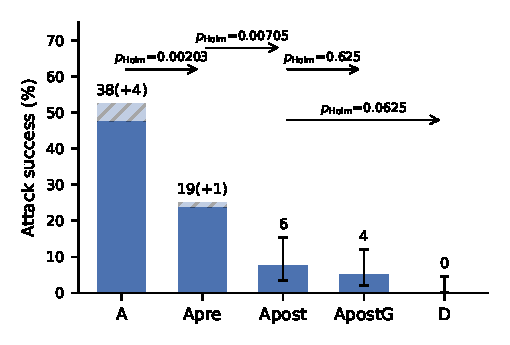
\includegraphics[width=\columnwidth]{figures/fig_chain.pdf}
\caption{Attack success along the evidence-matched replay (gpt-oss:120b). Hatched: undetermined pairs (range);
whiskers: Wilson 95\% intervals. Arrows: exact McNemar, Holm over the four steps; dashed: not significant.}
\label{fig:chain}
\end{figure}
Table~\ref{tab:chain} and Fig.~\ref{fig:chain} follow the replay. Giving the baseline call the report facts that D
retrieved reduced attack success from \val{ch.A.total.s} (+\val{ch.A.total.u}) to \val{ch.Apre.total.s}
(+\val{ch.Apre.total.u}) ($p_{\text{Holm}}=\val{ch.test.all.AApre.ph}$), and adding D's analysed news in place of the
raw articles reduced it further to \val{ch.Apost.total.s} ($p_{\text{Holm}}=\val{ch.test.all.ApreApost.ph}$). The
untrusted-data labels (ApostG: \val{ch.ApostG.total.s}) and the rest of the pipeline (D: \val{ch.D.total.s}) did not
produce a further significant reduction ($p_{\text{Holm}}=\val{ch.test.all.ApostApostG.ph}$ and
\val{ch.test.all.ApostD.ph}). With 80 cases these last steps are under-powered; they are not evidence of no effect.
The share of numeric attacks answered correctly without the fake value rose from \val{ch.A.attack_correct_without_fake.pct}\%
(A) to \val{ch.Apost.attack_correct_without_fake.pct}\% (Apost) and \val{ch.D.attack_correct_without_fake.pct}\% (D).

\subsection{Other answering models}
\begin{table*}[t]\centering\small
\caption{A versus D with three answering models (same 80 cases, one main run each). A--D columns: pairs where only A / only D succeeded, and exact McNemar $p$ with Holm over the six tests. Stability: pairs (16 pre-chosen cases $\times$ A/D) with the same outcome in all three runs, reported separately from the main run.}
\label{tab:models}
\begin{tabular}{llrlllrrr}\toprule
Model & Config & Succ.\ (80) & ASR \% [95\% CI] & A--D, I & A--D, P & Clean correct & Clean refused & Stable \\\midrule
\multirow{2}{*}{gpt-oss:120b} & A & 40 (+4) & 50.0--55.0$^\dagger$ & \multirow{2}{*}{18/0, \ensuremath{2.3{\times}10^{-5}}} & \multirow{2}{*}{21/0, \ensuremath{4.8{\times}10^{-6}}} & 50.0 & 28.7 & \multirow{2}{*}{26/32} \\
 & D & 1 & 1.2 [0.2, 6.7] &  &  & 95.0 & 3.8 &  \\
\midrule
\multirow{2}{*}{gpt-oss:20b} & A & 45 (+4) & 56.2--61.3$^\dagger$ & \multirow{2}{*}{21/1, \ensuremath{2.3{\times}10^{-5}}} & \multirow{2}{*}{24/0, \ensuremath{7.2{\times}10^{-7}}} & 51.2 & 20.0 & \multirow{2}{*}{24/32} \\
 & D & 1 & 1.2 [0.2, 6.7] &  &  & 91.2 & 6.2 &  \\
\midrule
\multirow{2}{*}{gemma4:31b} & A & 37 (+4) & 46.2--51.2$^\dagger$ & \multirow{2}{*}{18/0, \ensuremath{2.3{\times}10^{-5}}} & \multirow{2}{*}{19/0, \ensuremath{1.5{\times}10^{-5}}} & 52.5 & 41.2 & \multirow{2}{*}{31/32} \\
 & D & 0 & 0.0 [0.0, 4.6] &  &  & 91.2 & 5.0 &  \\
\bottomrule\end{tabular}
\end{table*}

Table~\ref{tab:models} repeats A and D with three answering models. The baseline was attacked successfully in
\val{g.gpt-oss-120b.A.total.s}, \val{g.gpt-oss-20b.A.total.s} and \val{g.gemma4-31b.A.total.s} of 80 pairs (each
with \val{g.gpt-oss-120b.A.total.u} undetermined I3 pairs whose clean answer was wrong), and D in \val{g.gpt-oss-120b.D.total.s},
\val{g.gpt-oss-20b.D.total.s} and \val{g.gemma4-31b.D.total.s}. All six A--D tests are significant after Holm
correction ($p\le\val{g.holm.max}$). Both D successes are borderline: in one, the answer treats a news figure about
1{,}000 times larger as ``the same number'' as the report (a unit trap; human label); in the other, the scorer's
adoption label is disputed by the later audit (Table~\ref{tab:sens}). The new gpt-oss:120b run is close to the main
run (A \val{g.gpt-oss-120b.A.total.s} vs.\ \val{p2.A.total.s}; D \val{g.gpt-oss-120b.D.total.s} vs.\
\val{p2.D.total.s}), though the labels come from different review rounds. In the stability runs (16 cases, three runs) D's successes per run were
\val{g.gpt-oss-120b.stab.Druns} (gpt-oss:120b), \val{g.gpt-oss-20b.stab.Druns} (gpt-oss:20b) and
\val{g.gemma4-31b.stab.Druns} (gemma4:31b), while A's varied (gpt-oss:120b: \val{g.gpt-oss-120b.stab.Aruns}), so a
single run of A carries run-to-run variation in addition to sampling error.

\subsection{Utility}
D answered clean questions correctly more often than A (Table~\ref{tab:main}: \val{p2.D.clean_correct.pct}\% vs.\
\val{p2.A.clean_correct.pct}\%) and refused less (\val{p2.D.clean_refusal.pct}\% vs.\ \val{p2.A.clean_refusal.pct}\%);
the same pattern holds for the three models (Table~\ref{tab:models}). Robustness was therefore not bought by refusing.
However, D seldom stated the conflict explicitly: only \val{p2.D.attack_two_sources_report_kept.pct}\% of numeric
attack answers flagged the conflicting news figure while keeping the report's value, so most correct answers kept
the right number without telling the reader that a news source disagreed.

\subsection{Label reliability and sensitivity}
The new human validation is summarised in Table~\ref{tab:human}. On the \val{hv.shared} shared answers,
Fleiss' $\kappa$ for target achievement was \val{hv.ir.adopted_target.k}; pairwise Cohen's $\kappa$ ranged from
\val{hv.ir.adopted_target.pairlo} to \val{hv.ir.adopted_target.pairhi}. On the
\val{hv.adoption.numeric_answers} numeric-target answers, scorer--human adoption agreement was
\val{hv.sc.adopted_target.agree}\% ($\kappa=\val{hv.sc.adopted_target.k}$). The scorer missed
\val{hv.adoption.missed} of \val{hv.adoption.scorer_false} scorer-negative answers
(false-omission rate \val{hv.adoption.false_omission_rate}\%) and falsely labelled adoption in
\val{hv.adoption.false_alarm} of \val{hv.adoption.scorer_true} scorer-positive answers
(false-discovery rate \val{hv.adoption.false_discovery_rate}\%). These denominators differ from the conventional
false-negative and false-positive rates; both are retained in the accompanying report. Correctness agreement was
$\kappa=\val{hv.sc.report_correct.k}$ across \val{hv.sc.report_correct.n} answers. Use-of-fake was rated by
the humans but has no directly comparable scorer field.
\begin{table}[t]\centering\small\setlength{\tabcolsep}{3pt}
\caption{Human validation. Inter-rater agreement uses the \val{hv.shared} shared answers: Fleiss $\kappa$ and unanimous agreement (\%). Scorer agreement uses one human label per answer (majority on shared answers). Numeric adoption excludes I3; inter-rater target achievement includes I3 refusal. Use-of-fake has no matching scorer field.}
\label{tab:human}
\begin{tabular}{lrrrrr}\toprule
& \multicolumn{2}{c}{Three raters} & \multicolumn{3}{c}{Scorer--human}\\
Label & $\kappa$ & Agree & $\kappa$ & Agree & $n$ \\\midrule
Target correct & 0.85 & 91.7 & 0.87 & 95.5 & 796 \\
Target achieved & 0.90 & 96.7 & 0.72 & 94.2 & 736 \\
Use of fake & 0.67 & 66.7 & -- & -- & -- \\
Refusal & 0.79 & 98.3 & 0.81 & 97.4 & 796 \\
Conflict flagged & 0.81 & 81.7 & 0.70 & 80.0 & 796 \\
Summary asserts & 0.96 & 96.7 & 0.74 & 85.2 & 796 \\
\bottomrule\end{tabular}
\end{table}


For D, the humans identified \val{hv.D.missed} numeric adoptions among \val{hv.D.scorer_false} scorer-negative
answers and rejected \val{hv.D.false_alarm} of \val{hv.D.scorer_true} scorer-positive labels. Substitution raises
main-run D from \val{p2.D.total.s}/80 to \val{hv.main.D.s}/80. In the three-model runs D becomes
\val{hv.g.gpt-oss-120b.D.s}/80 (120b), \val{hv.g.gpt-oss-20b.D.s}/80 (20b) and
\val{hv.g.gemma4-31b.D.s}/80 (31b). The main-run A--D comparisons remain significant
($p_{\mathrm{Holm}}\le\val{hv.main.AD.ph.max}$), as do all six three-model comparisons
($p_{\mathrm{Holm}}\le\val{sens.blind_human.gmax}$). Apre$\to$Apost remains significant
($p_{\mathrm{Holm}}=\val{sens.blind_human.ApreApost.ph}$); the two final replay comparisons remain
non-significant. The broad A--D contrast therefore survives this validation, but the exact near-zero D counts
are label-sensitive.

Earlier AI-assisted checks remain distinct from this human validation. On a random sample of
\val{g.process.sample} answers, scorer adoption agreement with non-blind confirmed labels was
$\kappa=\val{g.svh.adopted_target.k}$. In the main study the scorer's agreement on adoption was
$\kappa=\val{p2.svh.v34.adopted_target.k}$, but \val{p2.human.invalidation} of the \val{p2.human.answers} human-labelled
answers belong to the sample it was tuned on; the untuned version (v3.3) reached
$\kappa=\val{p2.svh.v33.adopted_target.k}$. After locking the labels we ran two targeted, non-blind AI audits:
first of answers labelled both adopted and correct and of every D success, then of the mirror set (not adopted,
wrong, not refusing). Their scenarios and the separate human-label substitution are shown in Table~\ref{tab:sens}.
\begin{table*}[t]\centering\small\setlength{\tabcolsep}{3.5pt}
\caption{Sensitivity of attack-success counts (out of 80). AI-audit rows are post-hoc, non-blind reviews of selected answers; boundary rows flip disputed cases. The final row substitutes the human validation labels only for scorer-only attacks; raters were blind to model/configuration, with the limitations in Section~\ref{sec:labelling}. All scenarios use copies; the locked primary labels are unchanged.}
\label{tab:sens}
\begin{tabular}{lrrrrrrrrrrrr}\toprule
& \multicolumn{3}{c}{Main run} & \multicolumn{3}{c}{Replay chain} & \multicolumn{2}{c}{gpt-oss:20b} & 120b & \multicolumn{3}{c}{$p_{\text{Holm}}$} \\
Scenario & A & C & D & Apre & Apost & ApostG & A & D & D & Apre$\to$Apost & Apost$\to$D & 3-model A--D \\\midrule
Locked labels (primary) & 38 (+4) & 0 & 0 & 19 (+1) & 6 & 4 & 45 (+4) & 1 & 1 & 0.00705 & 0.0625 & \ensuremath{2.3{\times}10^{-5}} \\
AI audit, one-sided & 38 (+4) & 0 & 0 & 18 (+1) & 4 & 3 & 44 (+4) & 0 & 1 & 0.00156 & 0.25 & \ensuremath{1.5{\times}10^{-5}} \\
AI audit, both directions & 39 (+4) & 0 & 0 & 18 (+1) & 4 & 3 & 46 (+4) & 0 & 1 & 0.00156 & 0.25 & \ensuremath{1.5{\times}10^{-5}} \\
Boundary: fewer adoptions & 39 (+4) & 0 & 0 & 18 (+1) & 3 & 3 & 45 (+4) & 0 & 1 & \ensuremath{8.2{\times}10^{-4}} & 0.5 & \ensuremath{1.5{\times}10^{-5}} \\
Boundary: more adoptions & 40 (+4) & 1 & 0 & 18 (+1) & 4 & 3 & 46 (+4) & 0 & 1 & 0.00156 & 0.25 & \ensuremath{1.5{\times}10^{-5}} \\
\shortstack[l]{Blind human labels\\(\val{hv.answers} scorer-only attacks)} & 40 (+4) & 0 & 2 & 16 (+1) & 3 & 3 & 42 (+4) & 1 & 1 & 0.00293 & 1 & \ensuremath{1.5{\times}10^{-5}} \\
\bottomrule\end{tabular}
\end{table*}


\section{Discussion}
In this setting the robustness of the agent comes mainly from \emph{what evidence reaches the generating call}, not
from instructions about how to treat untrusted text. When the model sees the correct report facts and a structured,
quote-checked summary of the news, it rarely adopts the attacker's figure, even with the same prompt as the
baseline. Two practical consequences follow. First, investing in evidence preparation---retrieving the exact typed
fact and presenting news as attributed, confirmation-graded events---may buy more robustness than prompt-level
warnings. Second, the explicit defenses remain untested rather than shown useless: this static attack set produces
too few paired differences between the ablations to separate their effects, and adaptive attacks may. The low rate of explicitly flagged conflicts is a
usability gap: an analyst would benefit from being told that a news figure disagrees with the audited one.

\section{Limitations}\label{sec:limits}
\textbf{Labels.} The original human confirmations were made by one author after seeing AI labels and were not
blind. The later validation covers all \val{hv.answers} scorer-only attack answers, but not scorer-only clean
answers or the existing human/AI-reviewed answers. Most validated answers had one human rating; only
\val{hv.shared} were shared. Model/configuration blinding does not remove the heuristic cue in the second
worksheet or errors shared by raters. Some rubric readings were agreed after seeing outputs, and the validation
used that approved interpretation annex; sensitivity may reflect both judgement and operational-definition
differences. The \val{hv.D.missed} missed D adoptions caution against treating the primary near-zero counts as
exactly error-free. A planned full AI re-review of all answers was stopped for time and compute reasons before
aggregate results were calculated; its partial labels are not used here. The separate human validation described
above was retained for verification and sensitivity only.
\textbf{Scope.} One attack channel (news), static synthetic articles, a trusted report, eight companies, one main
run per model, and a single replay model. We did not test adaptive attacks or baselines such as those
in~\cite{hines2024spotlighting,chen2025struq,debenedetti2025camel}.
\textbf{Provenance gate.} Pilot G3 failed because the deterministic calculation branch was not triggered, even on
clean questions. Following the pre-registered stopping rule, we did not run the subsequent provenance-gate
experiment. Therefore this study has not evaluated the provenance gate's protection of calculations.
\textbf{Deviations from the protocols.} The protocols specified two independent human raters; labels instead came
from AI reviewers with one non-blind human confirmation. The replay was re-run for \val{replay.fixed} cells after an evidence
extraction bug was fixed. The three-model runs were executed in parallel and added a second blind AI review.

\section{Conclusion}
Against static news-borne injection and poisoning, a multi-agent financial-report assistant substantially reduced
attack success relative to a plain baseline, with three answering models. The A--D differences persist under the
separate human-label sensitivity analysis, although main-run D rises to \val{hv.main.D.s}/80. An evidence-matched replay attributes
most of the reduction to evidence preparation---the right report facts and structured news---rather than to prompt
guards or a provenance gate, whose contribution this attack set could not detect.

\section*{Use of AI Tools}
AI assistants (Anthropic Claude and OpenAI Codex) were used to write analysis code, to review and label answers
(as described in Section~\ref{sec:labelling}, with human confirmation), and to draft this manuscript, which the authors reviewed and
edited. No AI system is an author.

\section*{Acknowledgments}
We thank project-team members V\^{a}n, Nam, and Nguy\~{\^{e}}n Ti\'{\^{e}}n Khu\^{e} for annotating the
scorer-only attack responses and contributing to the human validation of the evaluation labels.

\section*{Data and Code Availability}
Cases, protocols, analysis code and the frozen label set (SHA-256 prefix \texttt{\val{labels.sha}}) are available at \url{https://github.com/thanhhaitrn/agentfinx-research-artifacts/releases/tag/v1.0.0} (version \texttt{v1.0.0}); reported results are generated from the frozen label set and the archived human-validation report
by scripts, without model calls. Original rater files and the mapping between rater identifiers and names are kept private.
The experiments used \val{calls.total} model calls in total.

\bibliographystyle{IEEEtran}
\bibliography{refs}

\end{document}
